% CVPR 2027 submission draft. Template: https://github.com/cvpr-org/author-kit
\documentclass[10pt,twocolumn,letterpaper]{article}

\usepackage[review]{cvpr}
%% This file contains a number of tweaks that are typically applied to the main document.
%% They are not enabled by default, but can be enabled by uncommenting the relevant lines.


%%
%% Official support for 2-column teaser figure
%%
\usepackage{cuted} %< for strip environment

%%
%% For auto-referencing of figures (see fig/teaser.tex and \label{} therein) 
%%
\usepackage{currfile} %< for \currfilebase macro

%%
%% caption and (global) spacing overrides
%%
\usepackage{caption} %< for "\captionof" commands (teaser)
% \setlength{\abovecaptionskip}{.5em} % space above caption
% \setlength{\belowcaptionskip}{1em} % space below caption

%%
%% Inline annotations; for predefined colors, refer to "dvipsnames" in the xcolor package:
%% https://tinyurl.com/overleaf-colors
%%
\newcommand{\red}[1]{{\color{red}#1}}
\newcommand{\todo}[1]{{\color{red}#1}}
\newcommand{\TODO}[1]{\textbf{\color{red}[TODO: #1]}}
%%
%% Disable for camera ready / submission by uncommenting these lines:
%%
% \renewcommand{\TODO}[1]{}
% \renewcommand{\todo}[1]{#1}

%%
%% Work harder in optimizing text layout. Typically shrinks text by 1/6 of page, enable
%% it at the very end of the writing process, when you are just above the page limit.
%%
% \usepackage{microtype}

%%
%% Fine-tune paragraph spacing.
%%
% \renewcommand{\paragraph}[1]{\vspace{.5em}\noindent\textbf{#1.}}

%%
%% Globally adjusts space between figure and caption.
%%
% \setlength{\abovecaptionskip}{.5em}

%%
%% Allows "the use of \paper to refer to the project name"
%% with automatic management of space at the end of the word.
%%
% \usepackage{xspace}
% \newcommand{\paper}{ProjectName\xspace}

%%
%% Commonly used math definitions.
%%
% \DeclareMathOperator*{\argmin}{arg\,min}
% \DeclareMathOperator*{\argmax}{arg\,max}

%%
%% Tighten underline.
%%
% \usepackage{soul}
% \setuldepth{foobar}

%%
%% Reconfigure paragraph (tweaks spacing)
%%

\usepackage{booktabs}
\usepackage{multirow}
\usepackage{amsmath}
\usepackage{tikz}
\usetikzlibrary{arrows.meta,positioning,fit}
\usepackage{xspace}
\usepackage{listings}
\renewcommand{\ttdefault}{lmtt}  % Courier (pcr) is unavailable under XeTeX; use Latin Modern Mono for code
\usepackage{upquote}
\lstset{basicstyle=\ttfamily\scriptsize, breaklines=true, columns=fullflexible, upquote=true,
  keepspaces=true, extendedchars=true, frame=none, xleftmargin=0pt,
  literate={"}{{\textquotedbl}}1}
\newcommand{\astra}{\textsc{Astra}\xspace}
\newcommand{\ours}{\textsc{ReSolve}\xspace}
\newcommand{\code}[1]{\texttt{\small #1}}

\definecolor{cvprblue}{rgb}{0.21,0.49,0.74}
\usepackage[pagebackref,breaklinks,colorlinks,allcolors=cvprblue]{hyperref}

\def\paperID{Draft}
\def\confName{CVPR}
\def\confYear{2027}

\title{ReSolve: Verified Mechanical CAD Edits\\and Linked Vector Drawings}

\author{Research working draft}

% Generated from completed local BenchCAD artifacts. Do not edit numeric results manually.
\newcommand{\onlineTrain}{492}
\newcommand{\onlineValid}{44}
\newcommand{\onlineTest}{126}
\newcommand{\onlineReferenceValid}{125}
\newcommand{\onlineMainRows}{Base, strict interface & 0 & 0 & 0 & 0 \\
Base, bare-list transport control & 56 & 0 & 1 & 0 \\
Fresh online-pair QLoRA & 77 & 12 & 18 & 12 \\}
\newcommand{\onlineCategoryRows}{T1 & 31 & 11 & 11 \\
T2 & 18 & 1 & 1 \\
T3 & 18 & 0 & 0 \\
T4 & 34 & 0 & 0 \\
T5 & 25 & 0 & 0 \\}
\newcommand{\onlineResultsDiscussion}{The trained model produces 77/126 applicable patches and 12/126 exact target ASTs. Of 125 independently valid STEP references, 39 predictions build valid solids, 18 reach IoU $\geq0.95$, and 12 reach strict IoU $\geq0.99999$ (9.6\,\%). The bare-list base control builds 3 solids, with 1 broad and 0 strict matches. Thus the experiment exposes a substantial remaining gap: most held-out edits fail to produce the reference geometry, particularly beyond literal-parameter changes.}
\newcommand{\onlineOperationalDiscussion}{Independent reference readback finds 125/126 valid target solids. One released rivet reference is invalid and is excluded from the geometric success denominator, while all task outputs remain reported. For the trained run, 39 cases are geometrically scored, 37 have execution errors and 49 have invalid patches; there are 0 timeouts and 0 Boolean-comparison errors. The observed code failures include invalid feature operations and damaged source coordinates; they are distinct from valid solids with low IoU.}

% Generated from completed H100 evaluation artifacts.
\newcommand{\cudaRows}{CUDA base & 0 & 0 & 0 & 0 \\
CUDA base, list wrapper & 47 & 0 & 0 & 0 \\
CUDA final LoRA & 61 & 16 & 19 & 15 \\}
\newcommand{\cudaSummary}{The final CUDA adapter yields 61/126 applicable patches and 16/126 target AST matches. Against 125 valid released STEP solids, 36 predictions execute, 19 meet broad IoU and 15 meet strict IoU (12.0\,\%). There are 65 invalid patches, 24 execution errors, 0 timeouts and 0 comparison errors; the same invalid released reference is excluded from the geometry denominator.}
\newcommand{\cudaAbstract}{A subsequent three-epoch H100 LoRA run on the same retained split produces 61/126 applicable patches and 15/125 strict solid matches.}

% Generated from completed six-case FEM attempt artifacts.
\newcommand{\femExampleRows}{Mounting angle & 2.043e-06 & 7.484e-07 & 7.464e-07 & 0.259 & Geometry + response agree \\
Locator block & 5.185e-08 & 3.742e-08 & 3.742e-08 & 0.003 & Geometry + response agree \\
Rotated shaft & 5.287e-07 & 5.287e-07 & 5.291e-07 & 0.068 & Geometry + response agree \\
Propeller & 3.334e-07 & 5.242e-07 & 5.221e-07 & 0.409 & Geometry fails; response agrees \\
Pan-head screw & -- & -- & -- & -- & Not verified: mesh failure \\
Round flange & 1.208e-07 & 1.212e-07 & 1.212e-07 & 0.021 & Geometry fails; response agrees \\}
\newcommand{\femAuditSummary}{Five of six case triples yield 15 solved source/target/prediction configurations with compliance mesh changes below 5\,\%. Across their recorded meshes the largest normalized equilibrium/energy error is 8.20e-13; final CAD-to-mesh volume error is at most 1.39\,\%. Three predictions meet both strict geometry agreement and the local 10\,\% target-compliance agreement tolerance. The propeller and flange predictions fail geometry while meeting that response tolerance. The screw has no FEM response because its boundary mesh fails; this also affects the source and released target, so it is not attributed solely to the model.}


\begin{document}
\maketitle

\begin{abstract}
Editing a mechanical drawing is useful only when the underlying part changes as requested and the delivered views remain consistent. We study a CAD-first workflow that predicts a validated program patch, executes the edited CadQuery model, and exports linked SVG views. Our main experiment uses published BenchCAD edit pairs with a local family- and template-component-disjoint train/validation/test split. A fresh 1.5B QLoRA model is trained on \onlineTrain{} retained edits and evaluated on all \onlineTest{} retained held-out cases, using source-program equality and the author's released STEP solids. The adapter yields 77/126 applicable patches and 12 exact target programs; 12 of 125 valid released STEP references are matched strictly. \cudaAbstract{} We report executable solids and volume agreement separately, with a format-relaxed base-model control. A smaller, explicitly localized pilot provides 150 verified edit pairs and paired drawing sheets. Separate deterministic truss and plate controls demonstrate axial FEM equilibrium and clearance violations; those results are not attributed to the learned CAD model. The study measures code-conditioned editing and linked view generation, not drawing perception or general engineering safety. The release lacks physical operating conditions; a separate, explicitly scenario-defined 3D elasticity audit checks six illustrated source/target/prediction triples after training.
\end{abstract}

\section{Introduction}
\label{sec:intro}
Changing four mounting holes to six is a shape-editing problem: the hole pattern must change while the flange body, hole diameter and bolt-circle radius remain consistent. Similar requests remove a bracket flange, add a blind shaft slot or enlarge a bore. These operations require localized changes to three-dimensional geometry, and their effects should remain coherent across views. \Cref{fig:benchcad-reference} illustrates two complex released source/target pairs.

Executable CAD provides a structured representation for this task. A model can change a construction history rather than separately generate each rendered view. Yet executable code is only one level of success. A valid edited solid may have the wrong feature locations; a high global overlap score may hide those errors because the affected region is small. For visual-geometry research, the central question is how to evaluate the requested shape change as well as overall shape agreement.

We implement \ours, an instruction-guided program-editing pipeline with three complementary observations: patch and execution outcomes, agreement with reference solids, and source-relative changes in common-camera projections. A supervised language model reads native CAD and an instruction, emits an original-coordinate patch, and executes through a representation-specific backend. Four-view drawings are derived from the same solid. Visual evaluation therefore concerns the executed geometry; it is not an image-conditioning or drawing-perception experiment.

The primary experiment uses a completed Colab T4 run with a fresh Qwen2.5-Coder-3B model, trained on public paired edits from BenchCAD and CAD-Editor~\cite{benchcad2026,cadeditor2025}. The resulting 39 strict matches among 252 held-out tasks improve on the fresh base's one match, but only 39 of 139 executed outputs meet the strict threshold. We retain this failure gap as a substantive finding. A subsequent visual audit illustrates why global agreement cannot substitute for feature-sensitive evaluation.

Mechanical response provides a further, conditional observation. We apply finite-element checks to illustrative edits only after specifying units, material, fixtures and loads. These post-edit checks measure numerical and target-response consistency under synthetic test scenarios. They neither provide training feedback nor establish manufacturing safety.

\paragraph{Contributions.}
\begin{itemize}
\item A documented two-source executable CAD editing experiment, separating patch applicability, solid execution and reference agreement on every retained held-out task.
\item A source-relative multi-view diagnostic over saved edited solids, with a realistic mounting-hole example that exposes the difference between whole-shape similarity and localized edit agreement.
\item An auditable link between edited geometry, derived vector views and scenario-defined FEM fields, with explicit unavailable outcomes and analysis assumptions.
\end{itemize}
Our contribution is empirical evaluation and reproducibility. Standard supervised adaptation, program patches, projections and FEM are not claimed as individually new. Earlier hardware runs, localized transport pilots and deterministic structural controls are documented separately in the supplement.


\begin{figure*}[t]
\centering
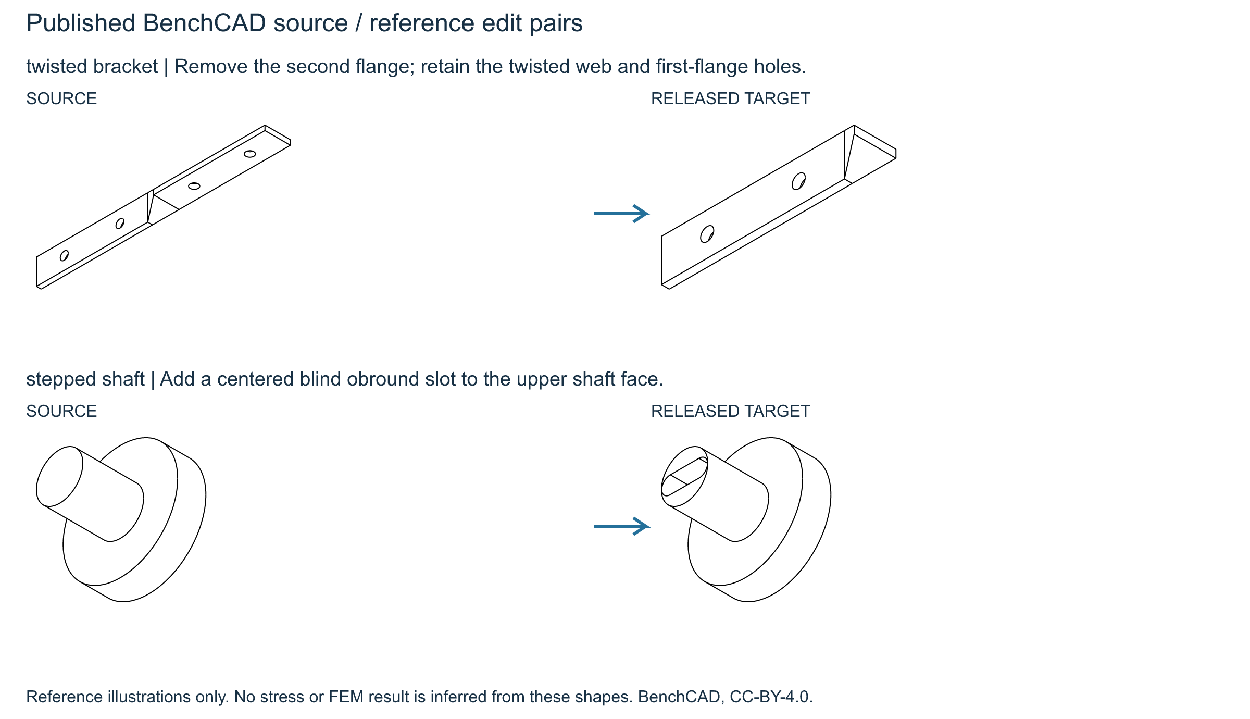
\includegraphics[width=0.93\textwidth]{figures/benchcad-reference-pairs.pdf}
\caption{\textbf{Published mechanical CAD edit pairs held out in the local protocol.} Top: remove the perpendicular end flange while preserving the twisted web and the first-flange holes. Bottom: add a centered blind obround slot to the upper cylindrical shaft section. These are source/released-target illustrations, not learned model predictions. Both views are exported from solids; shape appearance supplies no stress or FEM result; the separate FEM audit concerns the six actual predictions in the supplement.}
\label{fig:benchcad-reference}
\end{figure*}
\section{Related work}
\label{sec:related}
\paragraph{Executable CAD and editing.}
DeepCAD~\cite{wu2021deepcad} and Text2CAD~\cite{khan2024text2cad} model parametric construction histories. CAD-Editor~\cite{cadeditor2025} studies instruction-based sequence editing. BenchCAD~\cite{benchcad2026} supplies executable mechanical programs and published edit pairs, while neuralCAD-Edit~\cite{neuralcadedit2026} evaluates expert-requested edits. Our experiment reuses released supervision; a program-patch interface and execution check are implementation choices, not evidence that CAD editing itself is new.

\paragraph{Drawings and vector graphics.}
Drawing2CAD~\cite{drawing2cad2025} links vector views to CAD histories. DeepSVG~\cite{carlier2020deepsvg} and StarVector~\cite{rodriguez2025starvector} model vector graphics, and SVGEditBench~\cite{svgeditbench} benchmarks instruction-based SVG edits. Our learned experiment conditions on CAD code and exports SVG after execution. It therefore does not establish SVG-to-CAD extraction, image understanding, or robust annotation recovery from manufacturing sheets.

\paragraph{Physical evaluation.}
FEM-Bench~\cite{fem_bench} tests scientific code generation. CADEngBench~\cite{cadengbench2026} evaluates functional CAD edits and matched linear-static FEA. Geometry and FEA are complementary: the latter requires an analysis contract. We retain an explicitly specified axial-truss control but do not fabricate loads or materials for BenchCAD parts. A public runnable CADEngBench release was not verified in this work, so its reported FEA results are related work rather than our reproduced benchmark.

\section{Executable shape editing and evaluation}
\label{sec:method}
Figure~\ref{fig:mechanical-flow} links a realistic four-to-six mounting-hole request to the actual final 3B patch, edited solid and numerical fields. The source solid is an illustration of the program input, not a model input image.
\begin{figure*}[t]
\centering
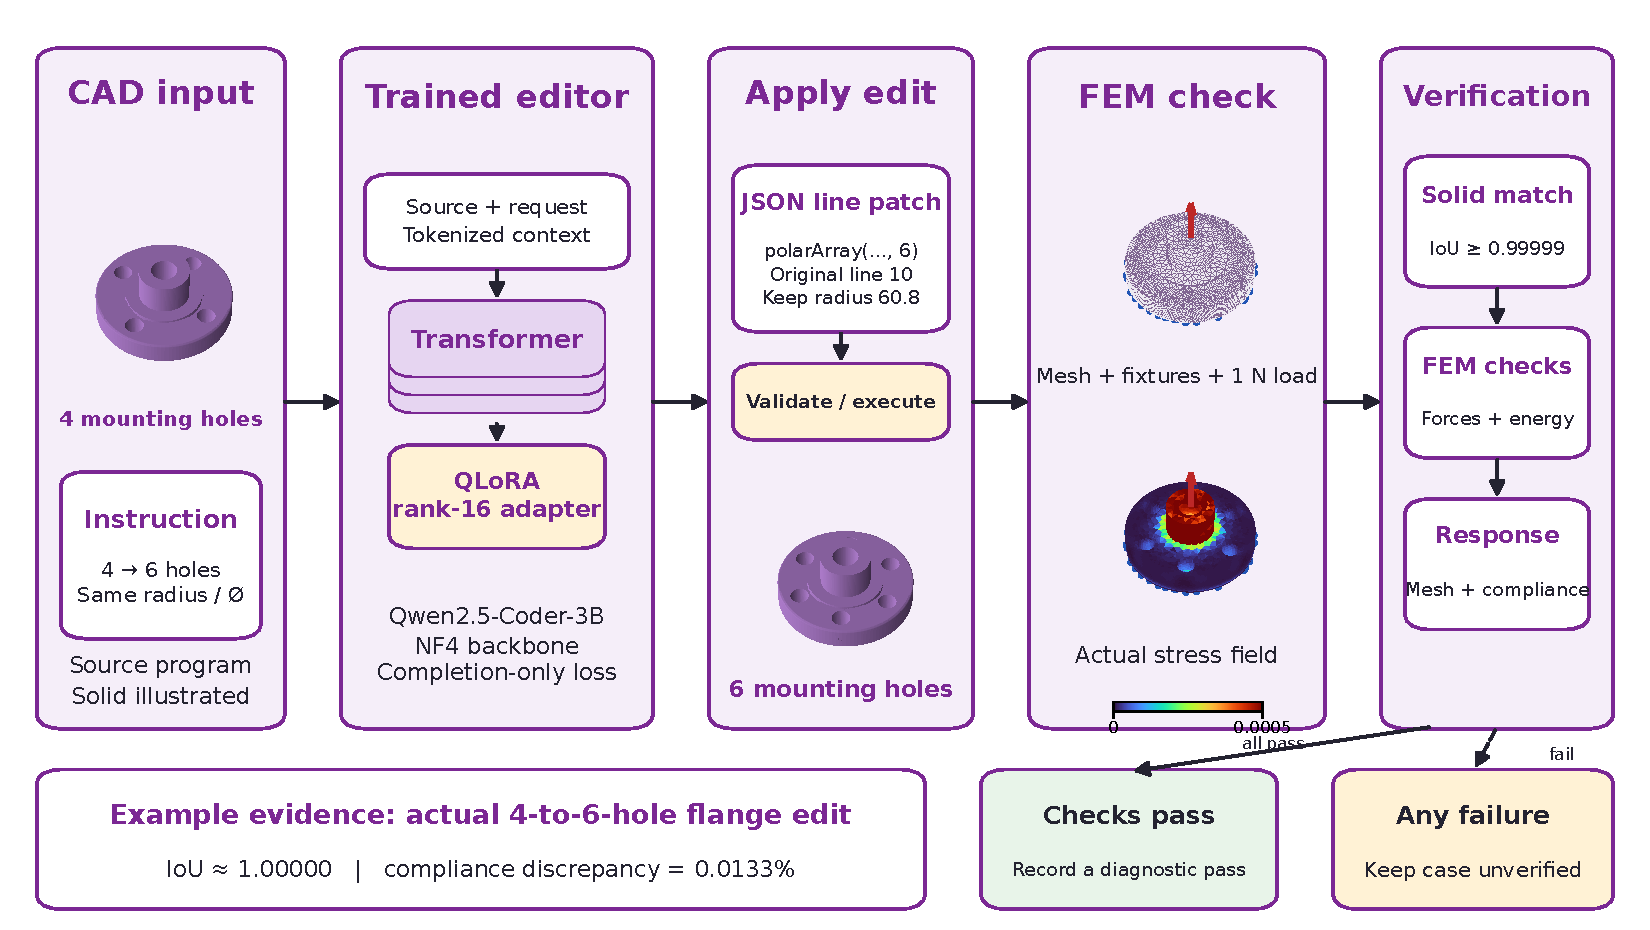
\includegraphics[width=0.98\textwidth]{figures/cad-fem-illustrated-architecture.pdf}
\caption{\textbf{Instruction-guided executable 3D editing.} Native CAD and text condition the trained editor. Validated patches produce the edited solid; views, solid comparison and optional FEM inspect that result. The shown flange is an actual final 3B prediction changing four holes to six at the same diameter and bolt-circle radius. Its saved tetrahedral mesh, fixture (blue), load (red) and von Mises field use a declared synthetic 1 N test; stress is clipped at p95 in MPa. FEM is an external diagnostic, not training supervision. Failed stages remain unverified.}
\label{fig:mechanical-flow}
\end{figure*}
\subsection{Model and patch contract}
Given source representation $C$ and instruction $u$, the model predicts patch $p$ and the executor returns $\hat C=\mathcal E(C,p)$. Each operation specifies a zero-based original line index, deletion count and replacement-line list. Operations must be typed, ordered, non-overlapping and in bounds. All coordinates address the original source. CadQuery syntax or native command-schema validation follows patch application.

We fine-tune Qwen2.5-Coder-3B-Instruct~\cite{hui2024qwen25coder} with NF4 double quantization and completion-only QLoRA~\cite{hu2022lora}. For supervised pairs $(C,u,p^\star)$, only answer tokens contribute to
\begin{equation}
\mathcal L_{\rm edit}=-\sum_{t\in\mathrm{answer}}\log P_{\theta,\phi}(p_t^\star\mid C,u,p_{<t}^\star),
\end{equation}
where $\theta$ denotes frozen base weights and $\phi$ the adapters. No image features, FEM loss, verifier reward or test-based checkpoint choice enters training. The architecture in Fig.~\ref{fig:mechanical-models} documents the native-representation branches.

\subsection{Execution and solid agreement}
The appropriate CAD backend builds a boundary-representation solid $\hat B$. Successful execution requires valid geometry, at least one solid and positive volume. The CadQuery executor permits a restricted set of imports and builtins, rejects private-attribute access and file I/O, and applies a 45-second per-case subprocess budget. This is defense in depth, not a general Python sandbox. Unsupported constructs and operational failures remain separate outcomes.

For target $B^\star$, volumetric intersection-over-union is
\begin{equation}
J_{\rm vol}=\frac{V(\hat B\cap B^\star)}{V(\hat B)+V(B^\star)-V(\hat B\cap B^\star)}.
\end{equation}
We use local broad and strict thresholds of 0.95 and 0.99999, respectively. Exact normalized program/sequence and patch matches are complementary diagnostics. None certifies engineering tolerances, preserved constraints or manufacturing suitability.

\subsection{Common-camera view and edit measurements}
We derive front, top, right and isometric views from each solid. The linked SVG sheets are CAD-derived views, not independently predicted images or production blueprints. For the focused visual audit, tetrahedral FEM is unnecessary: tessellated boundary surfaces are rasterized into binary orthographic silhouettes $S_v(B)$.

For each case and view $v$, source, target and available predictions share projection axes, image scale and center. Bounds use their union; no individual shape is recentered. We render 512- and 1,024-pixel square images with 0.3\,mm tessellation tolerance. This is a diagnostic camera contract, including available output bounds, rather than a predictor-independent camera benchmark.

For source solid $B$, define reference and predicted changes as
\begin{equation}
\Delta_v^\star=S_v(B)\oplus S_v(B^\star),\quad
\hat\Delta_v=S_v(B)\oplus S_v(\hat B),
\end{equation}
where $\oplus$ is binary exclusive-or. We report both silhouette IoU and edit-mask IoU $J_{\rm edit,v}=\operatorname{IoU}(\Delta_v^\star,\hat\Delta_v)$. Empty unions are undefined and excluded from the edit mean; nonempty unintended changes are retained. This exposes differences in the changed region, but cannot measure occluded/internal features or instruction semantics. Very small change masks are sensitive to rasterization; we disclose their effect rather than infer feature correctness from a scalar average.

\subsection{Conditional mechanical response audit}
FEM is applied only with an explicit physical contract. The illustrated BenchCAD scenarios assume mm/N/MPa units, $E=210{,}000$ MPa, $\nu=0.3$, a fixed lower 5\,\% surface band and an upper-band resultant of 1 N. These are declared test conditions, not recovered properties or operating loads. Native CAD-Editor examples lack established physical scale and are not assigned such results.

First-order tetrahedra solve small-strain 3D isotropic elasticity with $K_e=V_eB_e^TDB_e$ and fixed-degree elimination. We check finite solutions, anchored components, residuals, force/moment balance and $2U=\mathbf f^T\mathbf u$ to normalized error below $10^{-6}$. Refinement targets at most 5\,\% compliance change; a local response diagnostic compares predicted and target compliance within 10\,\%. This complements solid agreement and does not certify stress convergence or safety. Full contracts and saved fields appear in Appendix~\ref{sec:mechanical-fem}.

\section{Public data and local protocol}
\label{sec:data}
\paragraph{Two native representations.}
The primary split contains 2,540 training, 172 validation and 252 test tasks (Table~\ref{tab:data-primary}). BenchCAD provides CadQuery source/target programs, natural-language edits and released STEP references~\cite{benchcad2026}. Microsoft's CAD-Editor provides native six-bit sketch--extrude edit sequences~\cite{cadeditor2025}. We retain their different representations and backends rather than treating them as interchangeable histories. CAD-Editor reference solids are reconstructed locally through our decoder; they are not author-released STEP references.
\begin{table}[t]
\centering\small
\begin{tabular}{lrrr}
\toprule
Source & Train & Validation & Test \\
\midrule
BenchCAD & 492 & 44 & 124 \\
CAD-Editor & 2,048 & 128 & 128 \\
\midrule
Total & 2,540 & 172 & 252 \\
\bottomrule
\end{tabular}
\caption{\textbf{Retained primary data.} Counts define our local protocol, not an official benchmark split. Source-specific reference construction remains distinct.}
\label{tab:data-primary}
\end{table}

\paragraph{Provenance and isolation.}
BenchCAD is pinned at revision \texttt{5919f578ab09ec283603a082fab07c7639ab56eb} and declares CC-BY-4.0. Its 748 edit pairs yield 710 after family-based exclusion of pipe/electrical content. Family groups are joined when source/target AST templates match after numeric-literal masking; whole connected components are assigned to local splits before patch construction. The earlier retained test slice had 126 tasks; two additional pipe-related instructions are excluded from the primary experiment, yielding 124. CAD-Editor uses a documented subset of the public training/evaluation archive. Exact source/target connected components are isolated within each source; cross-source geometric ancestry is not established.

\paragraph{Retention and supervision.}
Token filtering and omissions are saved before training and evaluation. The primary model uses a 4,096-token context and a 768-token output cap. Training patches replay their normalized targets exactly. Comments and blank lines are removed when preparing CadQuery patches, avoiding supervision of parameter-comment edits as geometry. Published instructions are retained without adding answer-line hints. Native command sequences use their own schema and decoder.

\paragraph{Evaluation boundaries.}
BenchCAD's edit release was originally held out; repartitioning it for training changes the benchmark contract. We report local held-out agreement, not official leaderboard or official-test generalization. The primary denominator includes all 252 retained tasks, including six reference errors and one final-model worker timeout. Reference availability is tracked separately. A previously identified instruction/target conflict in a shaft-slot record illustrates that reference agreement does not certify natural-language compliance for every label. The supplement preserves the earlier split details and audits.

\section{Online editing experiments}
\label{sec:experiments}
\paragraph{Training.}
We start from a fresh 4-bit Qwen2.5-Coder-1.5B-Instruct conversion~\cite{hui2024qwen25coder} and train a QLoRA adapter~\cite{hu2022lora} using MLX on an Apple M5 with 16\,GB memory. The model conversion revision is \texttt{b3252a2f97102b1fb1571fec2c9b27219a8536be}. Seed 17, batch size one, learning rate $10^{-4}$ and the last eight transformer blocks are fixed. Adapters have rank 8, scale 20, no dropout, and cover attention and MLP linear projections in those blocks. Prompt tokens are masked from the loss. We run \onlineTrain{} optimizer steps, corresponding to one pass of the retained training rows, and use the final checkpoint. Validation is logged, not used to select among test-informed alternatives. Saved adapters are reloaded before evaluation.

\paragraph{Evaluation and metrics.}
Base and trained models receive the same original programs, published instructions and patch contract. Greedy decoding is capped at 512 new tokens. All \onlineTest{} retained test records are evaluated in the same fixed order. Applicability requires a valid patch and syntactically valid program; AST equality requires the executed program to match the published target's normalized syntax. Solid scoring executes the actual prediction and compares it with the released STEP reference. No gold edits repair a model prediction.

\begin{table*}[t]
\centering\small
\setlength{\tabcolsep}{8pt}
\begin{tabular}{lrrrr}
\toprule
System & Applicable & Target AST & IoU $\geq0.95$ & IoU $\geq0.99999$ \\
\midrule
\onlineMainRows
\bottomrule
\end{tabular}
\caption{\textbf{Local online-pair benchmark: counts out of \onlineTest{}.} All systems use the same family/template holdout. The transport control only wraps a bare JSON edit list into the required object, without changing coordinates or content. Timeouts and comparison errors remain separately disclosed; they are not measured incorrect geometry. This is a local split, not an official BenchCAD score.}
\label{tab:online}
\end{table*}

\paragraph{Transport control.}
The base model frequently emits a bare list of edits rather than the required object containing \texttt{edits}. We therefore add a deterministic diagnostic that wraps a syntactically valid bare list while preserving every operation. It makes 56 of 126 base predictions applicable, but none matches the target AST. This control distinguishes one schema mismatch from the remaining content and coordinate errors; it does not rewrite geometry, infer missing operations or correct indexing.

\paragraph{Results and operational coverage.}
\onlineResultsDiscussion
\onlineOperationalDiscussion
We keep base and trained outputs, patch errors, executed-solid measurements, reference hashes and category breakdowns. One seed and one model size cannot establish a robust scaling law or broad superiority over CAD agents. No official benchmark claim or statistical population failure rate is inferred from this local slice.

\begin{table}[t]
\centering\scriptsize
\setlength{\tabcolsep}{4pt}
\begin{tabular}{@{}lrrr@{}}
\toprule
Category & Cases & Target AST & Strict match \\
\midrule
\onlineCategoryRows
\bottomrule
\end{tabular}
\caption{\textbf{Trained results by published edit category.} Category IDs are retained from the source; counts are not pooled across different evaluation contracts.}
\label{tab:categories}
\end{table}

\paragraph{Additional H100 run.}
After the local experiment, available server compute supports a separately reported CUDA run. A fresh unquantized BF16 Qwen2.5-Coder-1.5B-Instruct model is trained on the identical 492 retained training rows for three epochs (1,476 updates) on one NVIDIA H100 NVL. PEFT adapters use rank 8, alpha 160 (scale 20), no dropout and the same seven attention/MLP projections in the last eight blocks. Seed, batch size, learning rate, prompt masking, context limit and greedy generation limit remain unchanged. We reload the final adapter and evaluate all 126 cases; no test-based checkpoint selection is performed. Different precision, software implementations and epoch counts prevent interpreting the comparison as an isolated hardware effect or an independent preregistered confirmation.

\begin{table*}[t]
\centering\small
\setlength{\tabcolsep}{8pt}
\begin{tabular}{lrrrr}
\toprule
System & Applicable & Target AST & IoU $\geq0.95$ & IoU $\geq0.99999$ \\
\midrule
\cudaRows
\bottomrule
\end{tabular}
\caption{\textbf{Additional three-epoch H100 experiment.} Counts cover the same 126 retained tasks and 125 valid references, using the unchanged local geometry thresholds. Both base and final model are decoded with the CUDA implementation; the wrapper control preserves predicted edit contents.}
\label{tab:cuda}
\end{table*}
\cudaSummary

\paragraph{Localized drawing pilot.}
The earlier 100-step adapter retained 92 training, 22 validation and 12 test examples after context filtering. All 12 held-out exact patches execute and match their references. Under a unique-substring line parser the base model already matches 11/12 solids. That result mainly improves transport formatting and cannot support a claim of advanced CAD reasoning. The online experiment uses published instructions without line hints, a fresh adapter and its own held-out families.

\section{Separate structural and clearance controls}
\label{sec:structures}
The full CAD benchmark above checks mechanical shape. A separate six-case FEM audit is described in the supplement. We retain a separately identified deterministic SVG route to show what physical or manufacturing checks require when a drawing does supply a contract. These synthetic controls are not training data or accuracy evidence for the learned BenchCAD model.

\paragraph{Axial trusses.}
An importer reads supported untagged truss geometry, section dimensions, material notes, nodal loads and supports. A bounded request interpreter generates validated SVG tree patches. Re-importing the actual patched SVG determines member lengths, orientations and axial areas. Linear-elastic pin-jointed elements use $EA/L$ stiffness; assembled displacements, stresses and reactions are recomputed. The numerical verdict checks equilibrium under small-displacement and nodal-load assumptions, not buckling, fatigue, joints or material strength.

\paragraph{Plate clearances.}
A separate importer recovers a rectangular boundary and circular-hole centres, diameters, thickness and stated limits. It computes overlap, edge distance and ligament. A faithful hole-enlargement request can reduce clearance below the printed minimum. A geometric violation is an engineering consequence of a correctly executed request, not necessarily an edit error; no continuum plate stress follows from a clearance score.

\begin{table}[t]
\centering\footnotesize
\setlength{\tabcolsep}{3pt}
\begin{tabular}{@{}lrr@{}}
\toprule
Route & Edits & Outcome \\
\midrule
Axial trusses & 20,008 & Equilibrium passes \\
Perforated plates & 19,992 & 699 clearance violations \\
\bottomrule
\end{tabular}
\caption{\textbf{Historical structural pipeline audit.} All 40,000 supported edits match their stored target trees. These counts describe a deterministic synthetic pipeline, not a learned CAD benchmark. The plate violations are faithful edits flagged by the geometric checker.}
\label{tab:structural}
\end{table}

For example, increasing all truss member depths from 20 to 40\,mm changes the recovered area and reduces peak axial stress from 11.861 to 5.930\,MPa under the same load. Enlarging plate holes from 10 to 16\,mm at fixed centres 20\,mm from a boundary reduces edge clearance from 15 to 12\,mm and fails a 15\,mm rule. These are distinct checks with explicitly stated assumptions. The saved audit and replayed source/edited SVGs remain separate from the new online training run.

\paragraph{When FEM is applicable.}
A stress, stiffness, buckling, thermal or contact request needs physical units, constitutive properties, loads and boundary conditions, followed by solver and mesh checks. The inspected BenchCAD edit pairs do not provide this analysis contract. We retain \emph{not evaluated} for the full released benchmark and distinguish the added six-case, synthetic-load FEM audit from validation under actual operating conditions.

\paragraph{Verification coverage.}
All six illustrated H100 cases are actual learned CAD program edits, followed by execution and comparison with released STEP targets. Each is now submitted to a separate 3D FEM response and mesh audit under the documented synthetic contract. The online benchmark and localized mechanical pilot check geometry; the plate controls check clearances. The six-case supplement solves 3D linear-elastic FEM problems, while the separate truss controls solve axial FEM equilibrium. Geometry agreement does not establish stress, stiffness or safety. FEM for a mechanical part would require an explicitly specified material, unit system, load case, supports and a validated mesh/solver setup, which are absent from these released edit pairs.

\section{Limitations and conclusion}
\label{sec:conclusion}
\ours studies instruction-guided executable 3D editing through program, solid, projected-change and conditional response measurements. The completed 3B adaptation improves local strict agreement to 39/252, while its large execution-to-agreement gap identifies remaining edit failures. The flange audit shows how localized visual changes can be missed by whole-shape similarity. Saved geometry and FEM fields make successful illustrative outcomes inspectable.

The model is code-conditioned, and deterministic projections do not establish learned visual perception. The visual audit covers six selected cases, with only four available final 3B outputs; it is not a benchmark-wide metric study. Projected masks miss hidden geometry, depend on rasterization and do not certify feature tolerances. Source-specific target reconstruction, known label defects, local repartitioning and unknown cross-source ancestry further limit the protocol. A single seed and standard QLoRA workflow cannot substantiate a new editing architecture or superiority to published CAD methods.

FEM checks use synthetic contracts on a small subset; they do not establish physical properties, stress convergence or operating safety. Stronger conclusions require matched CAD-editing baselines, repeated training runs, full-test feature/view evaluation and physical tasks with independent analysis contracts. Genuine drawing-conditioned editing remains future work rather than a capability of the current model.


{
    \small
    \bibliographystyle{ieeenat_fullname}
    \bibliography{refs}
}

\clearpage
\appendix
\section{Reproduction and evidence contracts}
\label{sec:appendix}
\paragraph{Online source.}
The \texttt{edit-bench} parquet is downloaded from \url{https://huggingface.co/datasets/BenchCAD/BenchCAD} at the revision stated in \cref{sec:data}. The original published split name is \texttt{edit\_bench}. Its 748 rows are not silently treated as 748 independent source shapes; grouping uses all original and edited programs before split assignment. Numeric literals are masked for template linkage; all records of a linked component retain one split.

\paragraph{Patch example.}
\begin{lstlisting}
{"edits":[
  {"start":5,"delete":1,
   "insert":["    .hole(6.0)"]}
]}
\end{lstlisting}
The zero-based line coordinate addresses the original code. A replacement list is required even for one line. Insertion uses zero deletions. The executor rejects overlapping operations and embedded newline characters. This example describes the interface, not an online gold answer.

\paragraph{Saved artifacts.}
The online dataset manifest pins the parquet checksum, split checksums, source IDs, categories and reference STEP hashes. The run manifest pins model revision, package versions, seed, optimization command, retained rows and omissions. The baseline and reloaded final adapter use identical test prompts. Predictions remain unmodified; the bare-list transport control is saved as a separate diagnostic. Geometry scores include every retained case, including invalid patches, code errors, unsupported constructs, timeouts and Boolean-comparison errors.

\paragraph{Evidence separation.}
The 150-pair localized pilot, 710-pair online protocol and historical 40,000-edit structural audit are different datasets and contracts. Their results are never pooled. The localized pilot's family test contains only 12 context-retained examples and gives line/number hints. The earlier single-source experiment evaluates 126 context-retained cases; the primary two-source 3B run evaluates 252 tasks. Structural FEM is only established for specified pin-jointed trusses.

\paragraph{Validation.}
Regression checks test multi-operation original-coordinate execution, insertion/deletion, malformed indexing, overlap rejection and comment preservation. Dataset checks require train/validation/test family and template-component disjointness, exact target-patch replay and pinned split hashes. Final adapters are reloaded for generation and checked for finite tensors. Reference STEP readback and all output geometry scores are retained. Source/reference illustrations are labeled as such and do not depict model predictions.

\section{Held-out model edit examples}
\label{sec:model-examples}
Figures~\ref{fig:example-success} and~\ref{fig:example-failure} show six actual predictions from the final three-epoch H100 adapter, alongside the input solid and released STEP target. These are illustrative cases selected after evaluation, not a random sample or additional test set; all 126 evaluated cases remain included in the reported aggregate results. We select three strict matches and three executable but geometrically incorrect edits to expose both supported behavior and remaining limitations. Each view is independently fitted to its panel, so apparent drawing size is not a dimensional comparison. Instructions and measured volume IoU accompany every row. These shape plates alone provide no FEM evidence; the separate scenario-defined audit below supplies the material, loading, support and solver records.

\begin{figure*}[p]
\centering
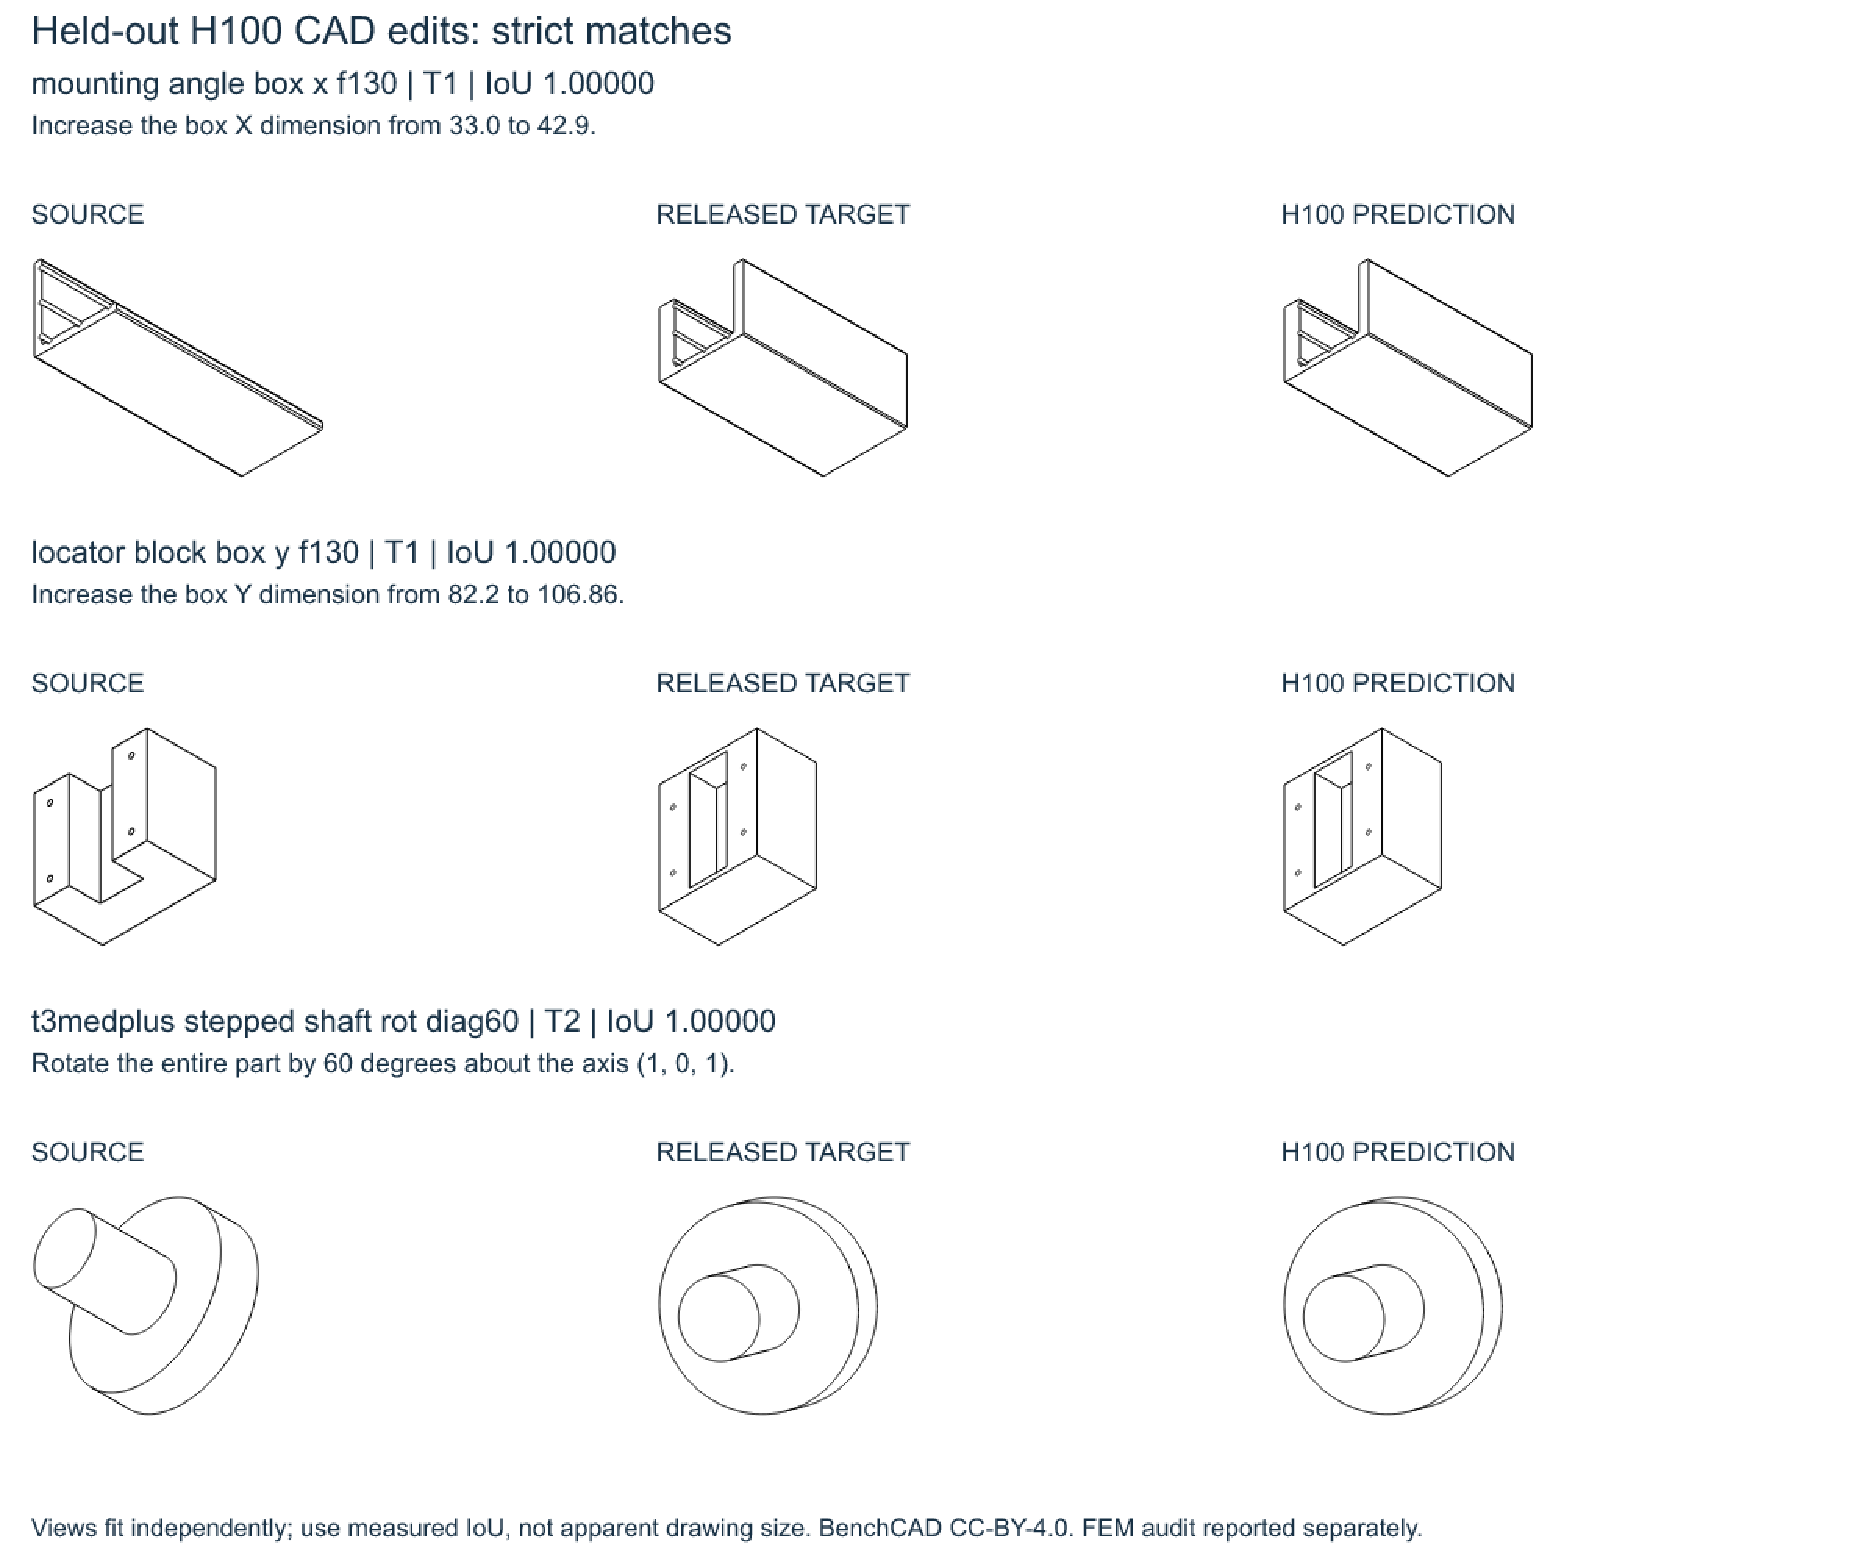
\includegraphics[width=0.98\textwidth]{figures/benchcad-model-examples-1.pdf}
\caption{\textbf{Three successful held-out H100 edits.} Rows show a mounting-angle dimension change, locator-block width change and a 60-degree stepped-shaft rotation. Columns contain the source, author's released target and actual final-adapter prediction. Each meets strict volume IoU $\geq0.99999$. These examples demonstrate reference agreement within the disclosed code-conditioned protocol; they do not certify general engineering correctness.}
\label{fig:example-success}
\end{figure*}

\begin{figure*}[p]
\centering
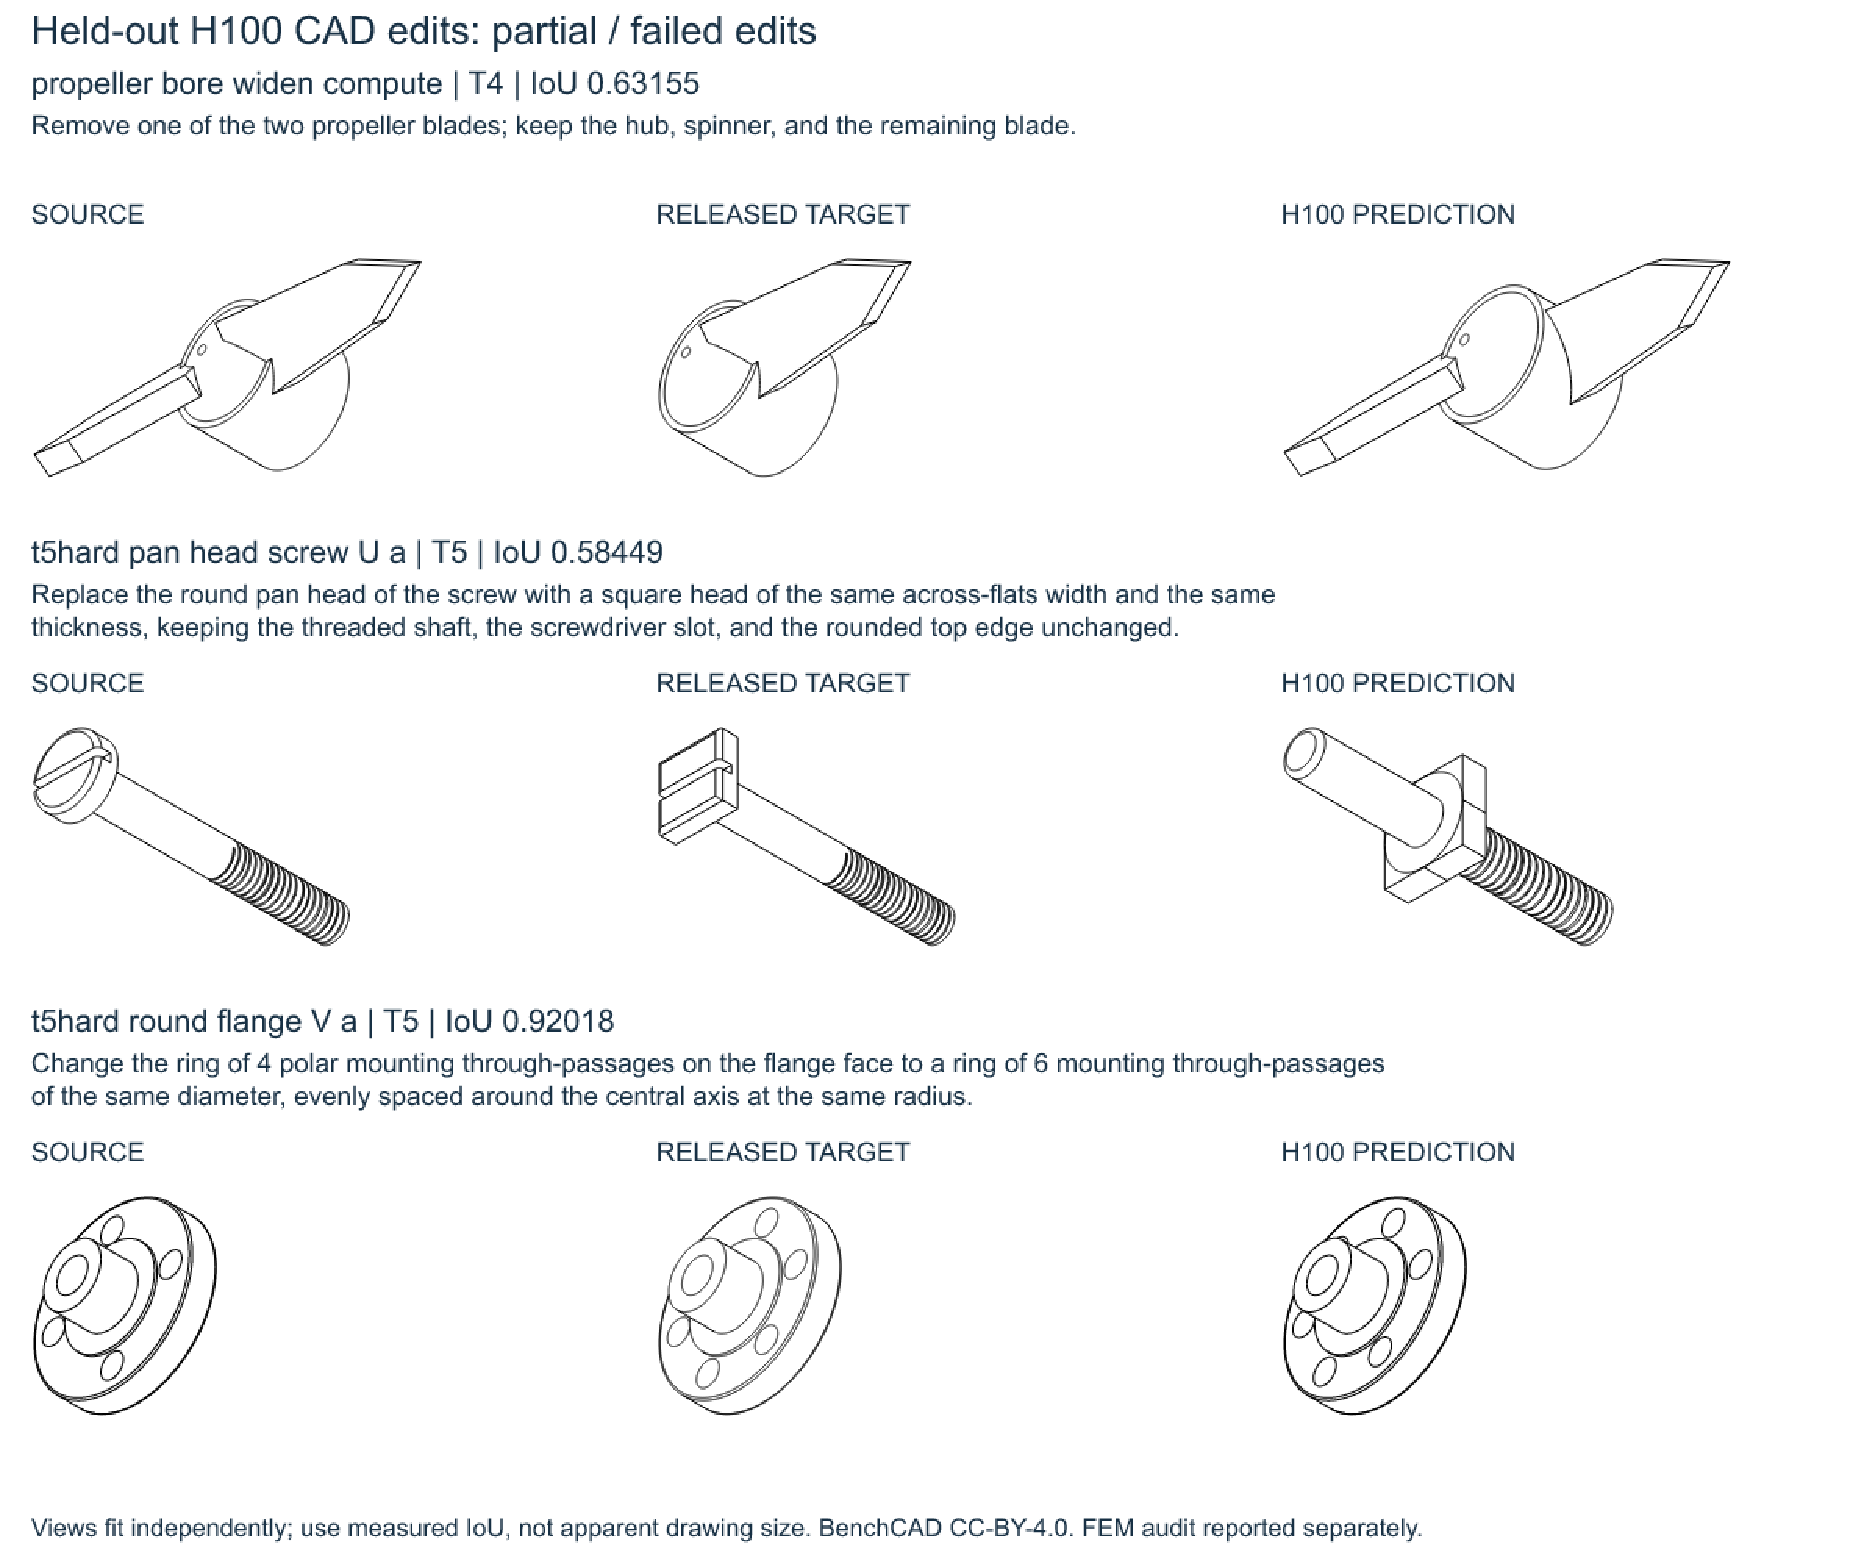
\includegraphics[width=0.98\textwidth]{figures/benchcad-model-examples-2.pdf}
\caption{\textbf{Three executable but incorrect held-out H100 edits.} Removing a propeller blade, replacing a screw head and changing a flange mounting-hole pattern yield valid solids but fail the strict reference threshold. Their volume IoUs are approximately 0.632, 0.584 and 0.920. Source, released target and model output remain separate; no reference operations repair these predictions. Small feature errors can remain important even when bulk volume overlap is high.}
\label{fig:example-failure}
\end{figure*}
\clearpage

\section{Scenario-defined FEM audit of mechanical edits}
\label{sec:mechanical-fem}
Figure~\ref{fig:fem-large-method} gives a visual walkthrough using two actual final 3B edited geometries; its mesh, displacement and stress panels are linked to saved solver fields.
\paragraph{Scope and physical contract.}
We attempt FEM on every source, released target and actual prediction in the six illustrated H100 cases: 18 configurations, independently of model training. The released dataset supplies no operating load case. We explicitly assume millimetres, newtons and MPa, a homogeneous isotropic material with $E=210{,}000$ MPa and $\nu=0.3$, and a 1 N resultant tensile test load. These are synthetic diagnostic conditions, not recovered material properties or certified operating conditions. All displacements are fixed at exterior mesh nodes in the lower 5\,\% of the shape's projected span along the analysis axis. A uniform vector traction is integrated over exterior triangles whose centroids occupy the upper 5\,\%; its area-weighted nodal forces sum to 1 N. The same geometric fixture rule is applied separately to each shape, rather than claiming identical world-coordinate contact patches. The shaft's fixture and load axis co-rotate with its requested 60-degree pose edit. Every case contract and STEP hash is saved before observing FEM responses.

\paragraph{Discretization and numerical checks.}
Gmsh~\cite{geuzaine2009gmsh} meshes the actual STEP geometry with first-order tetrahedra. A SciPy sparse implementation solves small-strain 3D isotropic elasticity,
\begin{equation}
\boldsymbol\epsilon=\tfrac12(\nabla\mathbf u+\nabla\mathbf u^T),\qquad
\boldsymbol\sigma=\lambda\operatorname{tr}(\boldsymbol\epsilon)\mathbf I+2\mu\boldsymbol\epsilon.
\end{equation}
The element stiffness is $K_e=V_e B_e^T D B_e$, with engineering shear strains. Dirichlet elimination solves the free-degree system. Checks require finite displacements, anchored connected components, positive strain energy, free residual, force and moment balance, and the identity $2U=\mathbf f^T\mathbf u$, each normalized numerical error below $10^{-6}$. An analytical uniform-tension cube agrees to numerical precision; load/modulus scaling and co-rotated-fixture tests also pass.

\paragraph{Mesh sensitivity and response comparison.}
We report compliance $C=\mathbf f^T\mathbf u$ in N\,mm. Global mesh sizes start at one twelfth and one eighteenth of the case's maximum bounding-box extent, with further refinement if the relative compliance change exceeds 5\,\%. The propeller source requires a third mesh. A local target-response diagnostic accepts compliance discrepancy at most 10\,\%, but this does not replace strict solid agreement. Stress fields and volume-weighted 95th-percentile von Mises values are retained for inspection; compliance convergence does not certify stress convergence. Clamp singularities, small feature errors, yield, buckling, fatigue, contact and actual-use safety are outside this experiment.

\begin{table*}[t]
\centering\scriptsize
\setlength{\tabcolsep}{4pt}
\begin{tabular}{lrrrrl}
\toprule
Example & Source $C$ & Target $C$ & Prediction $C$ & Discrepancy (\%) & Combined diagnostic \\
\midrule
\femExampleRows
\bottomrule
\end{tabular}
\caption{\textbf{Mechanical example FEM checks under explicit test scenarios.} Compliance values use N\,mm. Discrepancy compares the prediction with the target, with independently generated meshes. A response match is not sufficient for a correct edit. Dashes denote failed meshing, not zero displacement or an invented solver pass.}
\label{tab:mechanical-fem}
\end{table*}
\femAuditSummary
The incorrect screw output contains seven CAD solids, versus one in its target. Boundary meshing encounters intersecting facets/segments; a source-only finer-mesh and alternative HXT-mesher diagnostic also fails. No component fusion, thread removal, contact model or geometry repair is used to manufacture a solution. This case remains \emph{not verified}.

\section{Multi-source Colab training pipeline}
\label{sec:colab-pipeline}

\begin{figure*}[t]
\centering
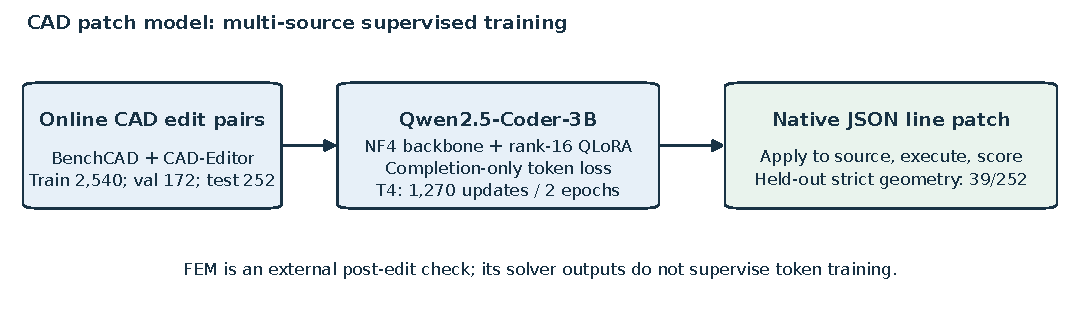
\includegraphics[width=0.98\textwidth]{figures/mechanical-trained-models.pdf}
\caption{\textbf{CAD editor architecture and supervised training.} Paired native CAD edits train the quantized Qwen2.5-Coder-3B backbone with completion-only QLoRA. Patches are applied and independently scored on held-out geometry; FEM remains an external post-edit check rather than a training loss.}
\label{fig:mechanical-models}
\end{figure*}
The reproducible extension uses paired edits from BenchCAD and Microsoft's CAD-Editor in their native representations. The prepared split contains 2,540 training, 172 validation, and 252 test records: respectively 492/44/124 CadQuery pairs and 2,048/128/128 native sketch--extrude pairs. Two additional pipe-related held-out instructions are excluded from this extension; the earlier 126-case experiment is unchanged. Exact source/target connected components are isolated within each source. Cross-source geometric ancestry is not established. Token-length filtering is recorded before training and evaluation.

A fresh Qwen2.5-Coder-3B-Instruct backbone uses NF4 double quantization and completion-only QLoRA: rank 16, alpha 320, the seven attention/MLP projections in the last twelve blocks, two fixed epochs, seed 17, learning rate $10^{-4}$, effective batch four, a 4,096-token context, and a 768-token output cap. The completed Colab T4 run uses microbatch one with four accumulation steps. Its saved manifest records \texttt{torch.bfloat16}; native BF16 hardware acceleration is not established. The final adapter is reloaded for greedy evaluation. Training completes 1,270 optimizer steps in 20,923.7 seconds with mean completion loss 0.2495. The adapter contains 9,977,856 trainable scalars; all 168 saved tensors are finite and their checksum matches the run manifest.

The model maps an instruction and original native CAD to an original-coordinate JSON line patch. Representation-specific schema and syntax checks precede execution. CadQuery patches are compared to released STEP targets; CAD-Editor command patches execute through a six-bit sketch--extrude decoder, with locally reconstructed target solids explicitly distinguished from author-released STEP files. Geometry and failure counts remain separate by source. Only examples with explicit material, unit, fixture, and load contracts proceed to tetrahedral FEM. Equilibrium, energy identity, mesh-volume fidelity, and compliance sensitivity checks precede a combined geometry/response diagnostic. FEM is an external post-edit tool, not a language-generated pass label or a solver reward used in training. Invalid patches and failed meshes remain unverified. The notebook saves adapters, manifests, predictions, geometry metrics, and numerical fields before downloading an artifact bundle.


\begin{table}[t]
\centering\scriptsize
\setlength{\tabcolsep}{3pt}
\begin{tabular}{lrrrr}
\toprule
Model / source & $n$ & Patch & Solid & Strict \\
\midrule
Fresh 3B base, all & 252 & 39 & 7 & 1 \\
Final 3B adapter, all & 252 & 173 & 139 & 39 \\
Final, BenchCAD & 124 & 91 & 65 & 25 \\
Final, CAD-Editor & 128 & 82 & 74 & 14 \\
\bottomrule
\end{tabular}
\caption{\textbf{Completed two-source Colab evaluation.} Patch denotes applicable schema/syntax; solid denotes successful execution/comparison; strict denotes volume IoU $\geq0.99999$. All retained tasks remain in $n$, including six reference errors and one final-model worker timeout. BenchCAD references are released STEP files; CAD-Editor targets are locally reconstructed native sequences.}
\label{tab:colab-completed}
\end{table}
\paragraph{Completed held-out results.}
The final adapter obtains 39/252 strict matches (15.48\,\%), versus 1/252 for the fresh base. Counts by source are 25/124 for BenchCAD and 14/128 for CAD-Editor. At IoU $\geq0.95$, the base and final adapter match 2 and 52 cases. Exact target-program/sequence agreement is 1 versus 32; exact patch agreement is 1 versus 31. No final generation reaches the output cap. The whole-worker timeout makes the scorer's reference-valid bookkeeping model-dependent (246 base, 245 final); we therefore use the complete held-out denominator, not 245 as a reference-valid test set. Different datasets, model size and training settings prevent treating this run as an isolated improvement over the earlier 1.5B experiment.

\paragraph{FEM of the new Colab adapter.}
We attempt the same six illustrative held-out instructions with the new model's unmodified patches. Four prediction/target pairs---mounting angle, locator block, rotated shaft, and round flange---pass strict geometry and the scenario-defined numerical, mesh-volume and compliance checks. Their relative compliance discrepancies are respectively 0.001123\,\%, 0.046691\,\%, 0.009141\,\% and 0.013270\,\%. The flange is now a strict match; the older H100 flange in Fig.~\ref{fig:fem-failure} remains an incorrect prediction from a different adapter. The new propeller patch fails syntax validation. The screw attempt leaves an incomplete pipeline directory; its resumed audit records failure, with no saved FEM solution establishing an original cause. Both cases remain unverified. Saved meshes and displacement/stress fields substantiate the four passes; source fields are from the separate earlier audit, not recomputed for this pairwise Colab audit. These are diagnostic test scenarios, not operating-safety evidence or full-benchmark FEM coverage.





\begin{figure*}[p]
\centering
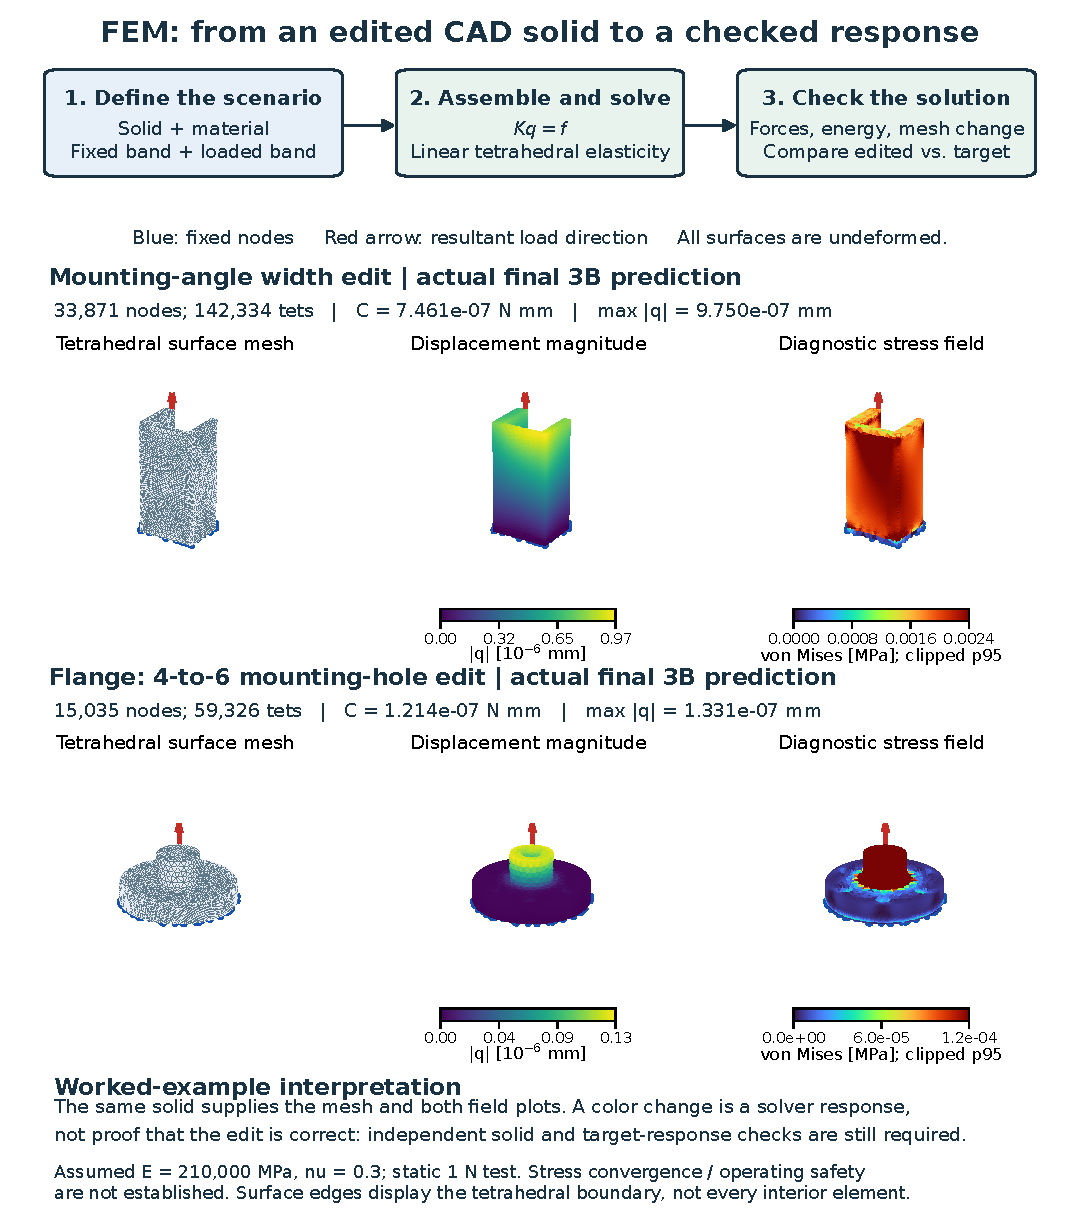
\includegraphics[width=0.98\textwidth]{figures/fem-method-worked-examples-large.pdf}
\caption{\textbf{Large FEM method walkthrough with actual mechanical edit examples.} The final 3B mounting-angle and six-hole flange predictions supply all meshes and fields. The left column displays the tetrahedral boundary mesh; the middle shows displacement magnitude; the right shows diagnostic von Mises stress, clipped at the per-example 95th percentile. Blue nodes are fixed and red arrows show the resultant load direction. Independent CAD/reference agreement, equilibrium, energy and mesh checks accompany these plots; stress color alone establishes neither correct editing nor strength. The listed values use each saved fine mesh and the disclosed synthetic static scenario.}
\label{fig:fem-large-method}
\end{figure*}



\begin{figure*}[p]
\centering
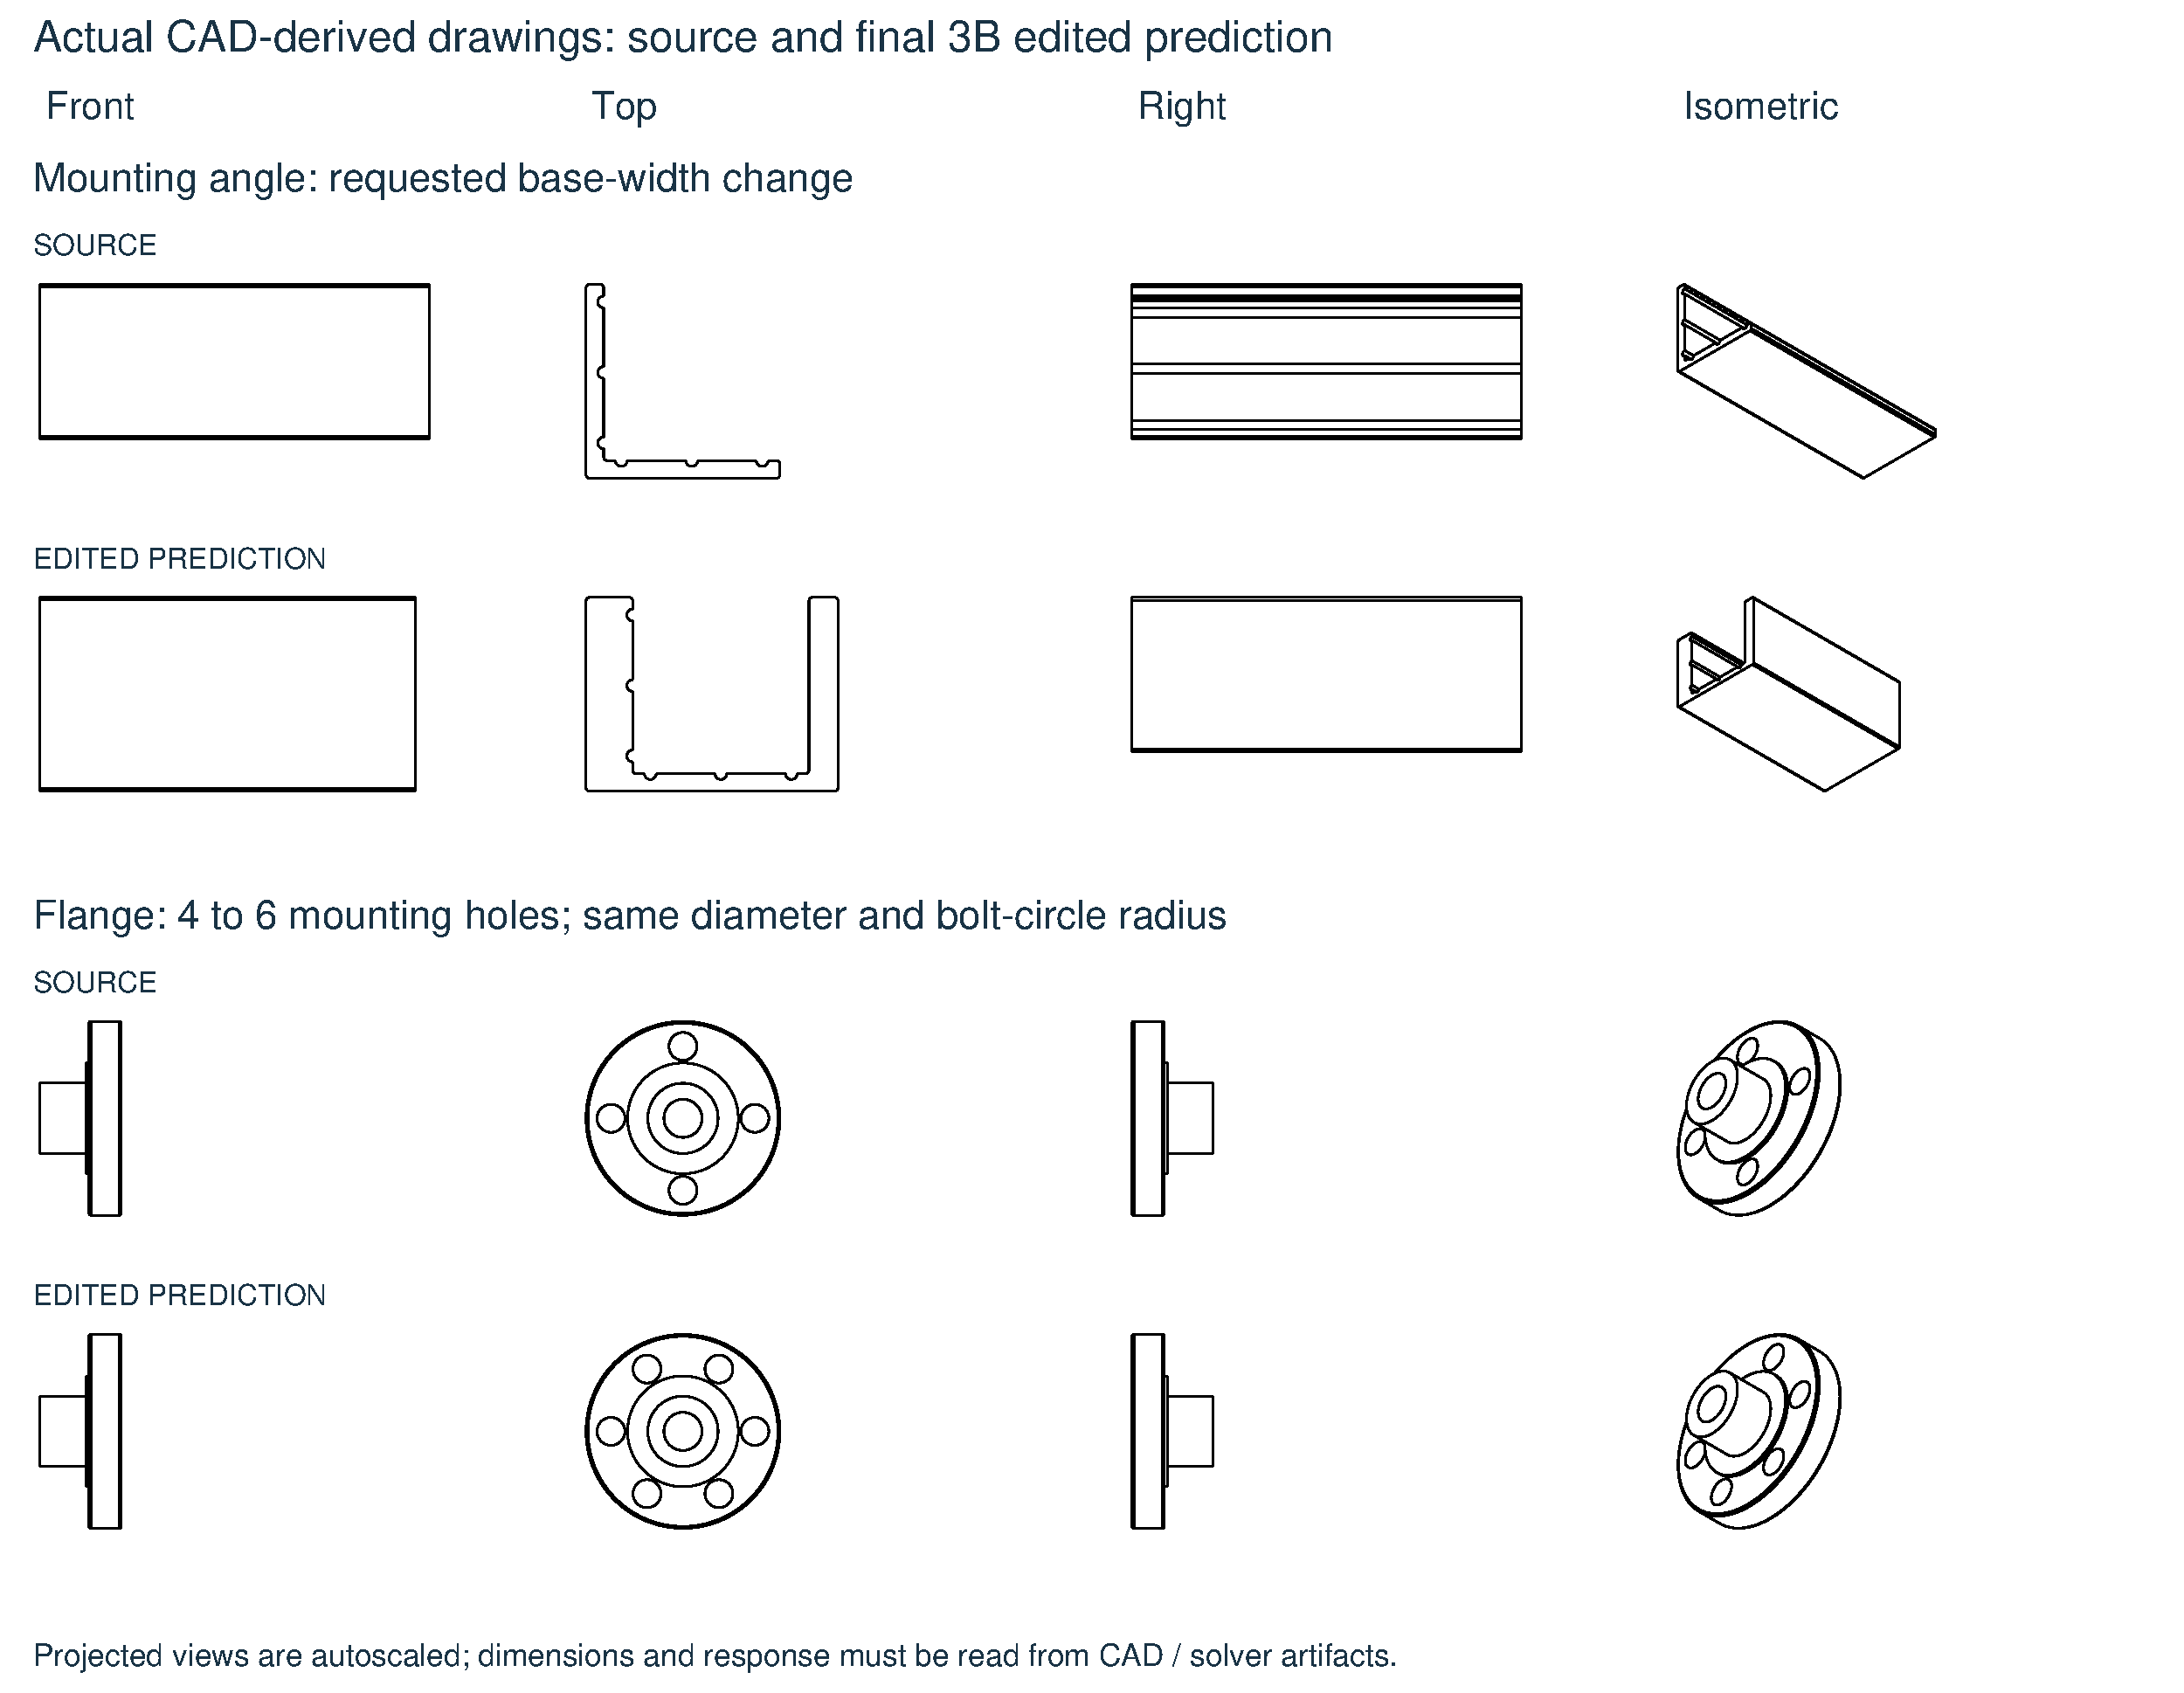
\includegraphics[width=0.98\textwidth]{figures/mechanical-linked-drawings.pdf}
\caption{\textbf{Linked engineering drawings from actual mechanical CAD solids.} Front, top, right and isometric views show the original and final 3B predicted mounting angle and flange. The flange edit changes four mounting holes to six equally spaced holes while retaining their diameter and bolt-circle radius; each panel is independently autoscaled. Both edited predictions pass the disclosed static geometry/FEM diagnostics. The views contain no inferred stress, production dimensions or hidden geometry repair.}
\label{fig:linked-drawings}
\end{figure*}

\begin{figure*}[p]
\centering
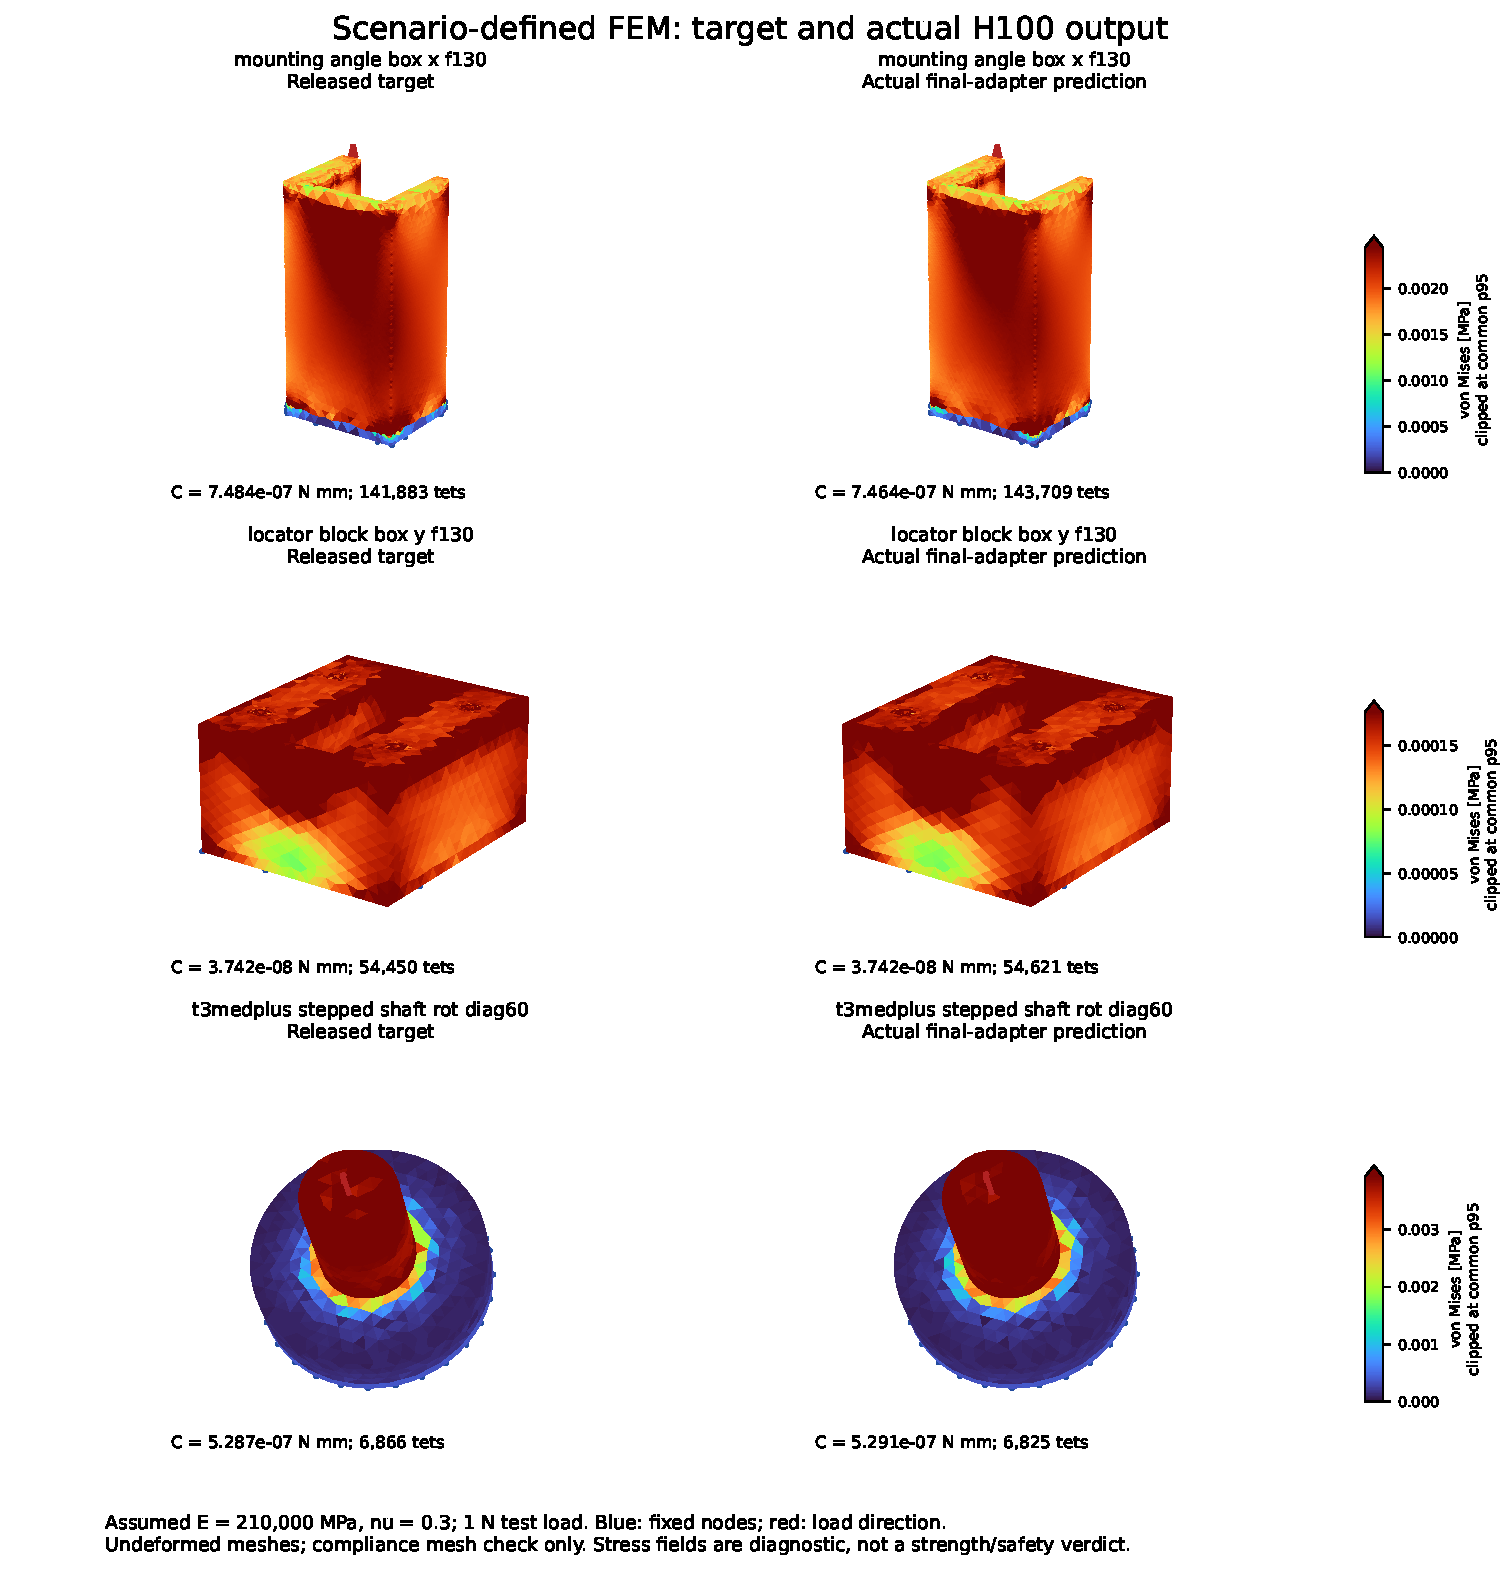
\includegraphics[width=0.97\textwidth]{figures/mechanical-fem-examples-1.pdf}
\caption{\textbf{Actual FEM fields for three geometry-matching H100 edits.} Released targets and model outputs use the documented synthetic test contracts. Blue points identify fixed nodes; arrows indicate the load direction. Undeformed surface stresses share a scale within each row, clipped above the common 95th-percentile value. Compliance passes the mesh-sensitivity check; stress colors are diagnostic rather than a strength verdict.}
\label{fig:fem-success}
\end{figure*}
\begin{figure*}[p]
\centering
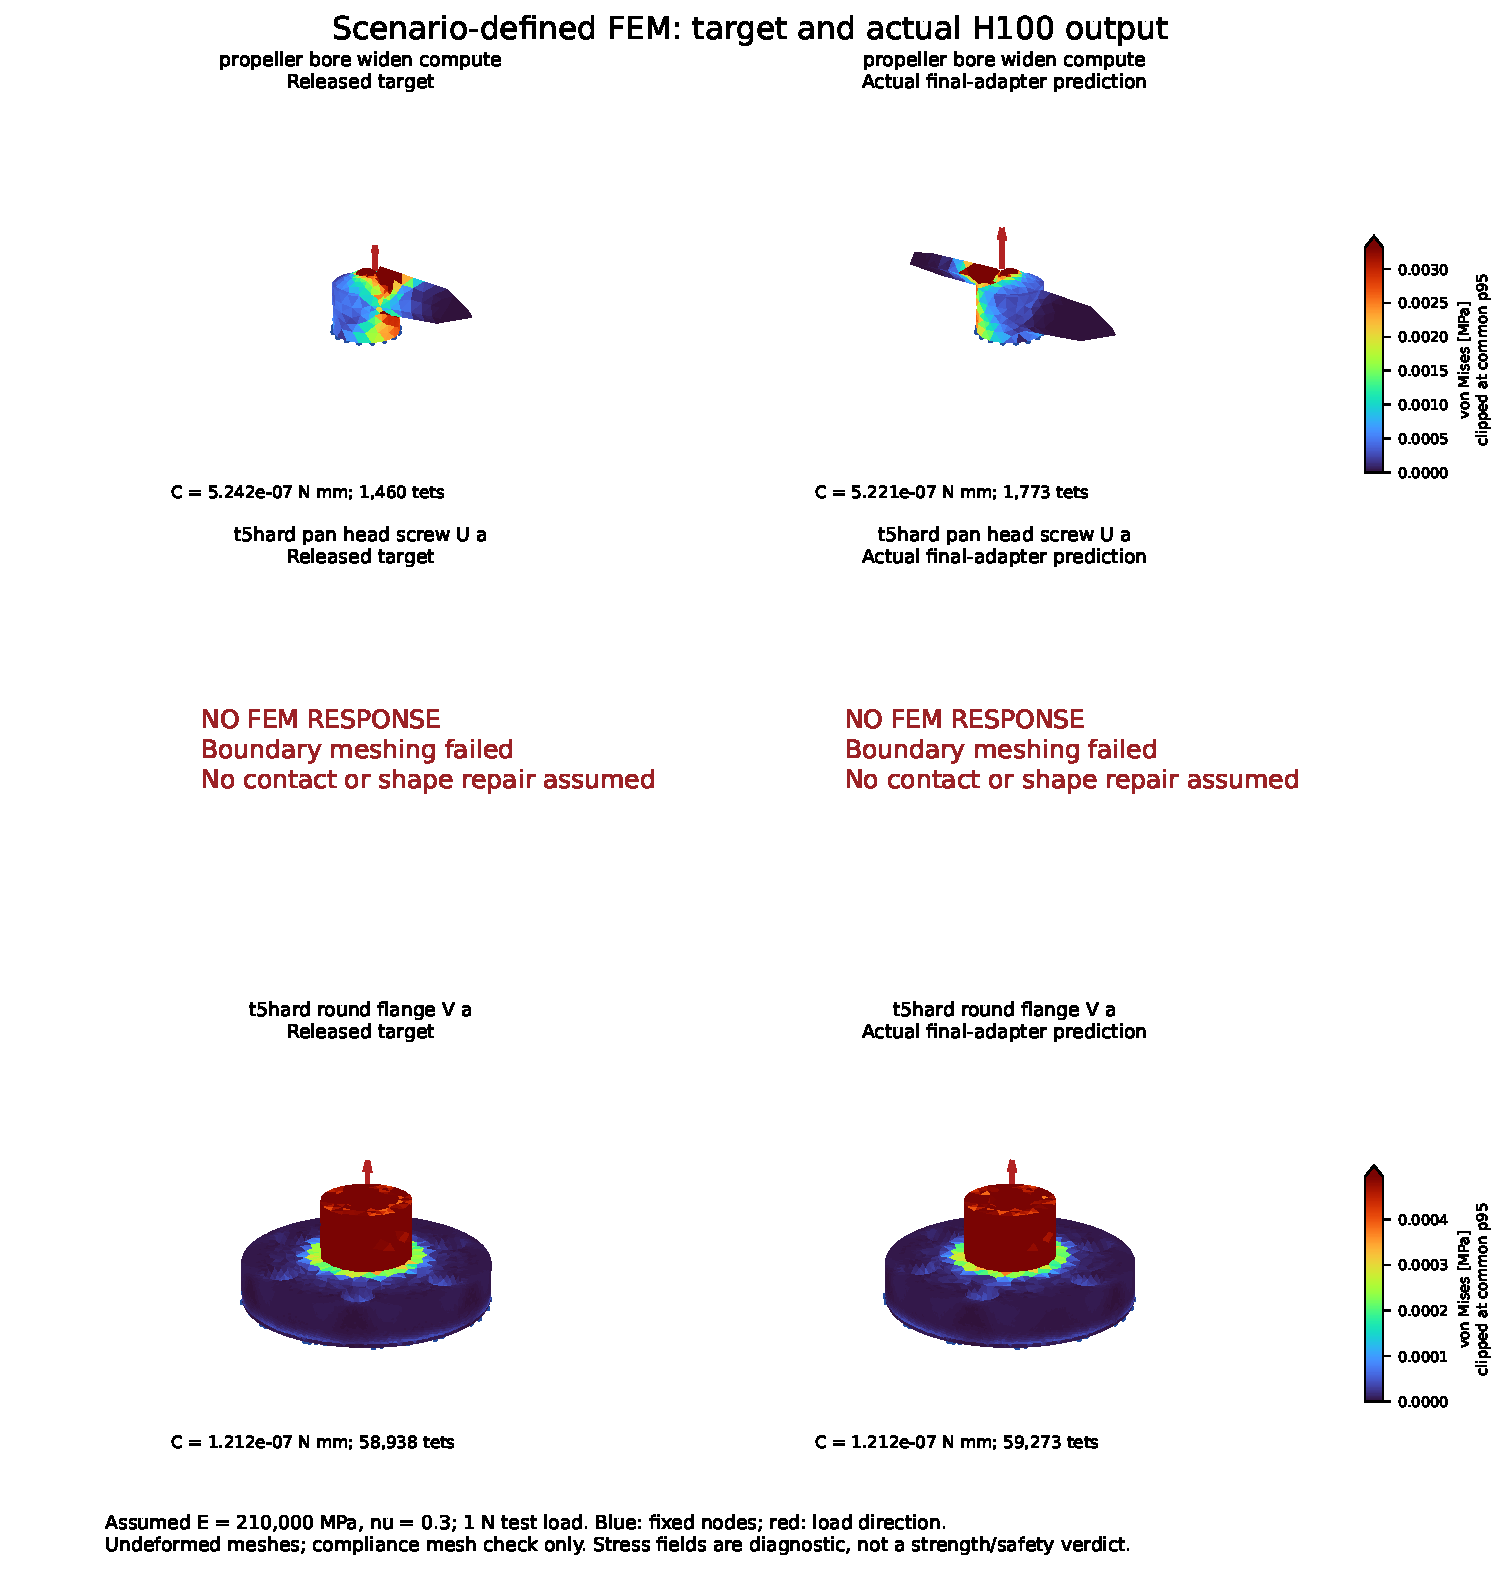
\includegraphics[width=0.97\textwidth]{figures/mechanical-fem-examples-2.pdf}
\caption{\textbf{FEM diagnostics do not replace edit fidelity.} Incorrect propeller and flange shapes produce similar compliance under the chosen test load, but fail strict reference geometry. The screw row has no FEM field because meshing fails; blank panels are explicitly marked. The same stress-scale and fixture conventions apply as in Fig.~\ref{fig:fem-success}.}
\label{fig:fem-failure}
\end{figure*}
\clearpage


\section{Focused visual audit details}
\label{sec:visual-audit}
The fixed case list comprises mounting angle, locator block, shaft, propeller, screw and round flange, previously chosen for illustration. Actual saved STEP files are tessellated, hashed and rasterized with the common-camera contract in Section~\ref{sec:method}. The earlier H100 adapter supplies six available solids; the final 3B adapter supplies four completed outputs. The adapters differ in model size, training corpus and optimization, so this subset is not a controlled model comparison. Failed/incomplete final outputs remain unavailable.
\begin{table}[h]
\centering\scriptsize
\begin{tabular}{lrrr}
\toprule
Saved outputs & Available & Silhouette IoU & Edit-mask IoU \\
\midrule
Earlier H100 & 6/6 & 0.911828 & 0.584674 \\
Final Colab 3B & 4/6 & 0.999993 & 0.874967 \\
\bottomrule
\end{tabular}
\caption{\textbf{Diagnostic projected means at 512 pixels.} Average views within cases, then cases with available outputs. Undefined empty-union edit views are excluded; unintended nonempty changes remain. Unequal availability and raster-degenerate masks prohibit reading this table as general comparative accuracy.}
\label{tab:visual-audit}
\end{table}
The mean absolute per-case change in edit-mask IoU between 512 and 1,024 pixels is 0.000113 for the older outputs and 0.000033 for the final available outputs. This small numerical change does not prove metric validity. For example, the flange's reference isometric change mask has only one pixel at 512 resolution. That degenerate view lowers the final flange's edit mean to roughly 0.5 despite essentially exact solid agreement, and contributes to the final aggregate of 0.874967. No mask-area threshold is introduced after inspecting results. Future full-test protocols should define minimum visible-change area or feature-aligned views in advance. Occluded features require solid/feature measurements; silhouettes cannot replace them. The raw report records every view's reference-change pixel count, two resolutions, all source/target/prediction STEP hashes and unavailable outcomes.

\section{Earlier single-source dataset protocol}
\label{sec:earlier-data}
\paragraph{Published pairs.}
We use the \texttt{edit-bench} configuration of \texttt{BenchCAD/BenchCAD}, pinned at revision \texttt{5919f578ab09ec283603a082fab07c7639ab56eb}. It contains 748 instruction/source/target pairs with original and target STEP data~\cite{benchcad2026}. The dataset declares CC-BY-4.0. Our downloaded parquet checksum and source-record identifiers are retained. Pipe, duct, fitting, manifold, valve, hose, resistor, circuit and PCB family names are excluded, removing 38 records and leaving 710 mechanical edit pairs.

\paragraph{Isolation before training.}
A complete mechanical family is one initial group. Families whose source or target ASTs share a template after masking numeric literals are joined into a component. Hash-ranked components are assigned approximately 70/10/20 to training, validation and test before normalization, patches or augmentation. This gives 533/50/127 pairs. Family and component identities are disjoint across splits; no target from a held-out family enters fine-tuning. Template isolation is conservative but does not prove all cross-dataset geometric ancestry is disjoint. The fresh run does not load the earlier mechanical adapter.

\paragraph{Context-limited coverage.}
We retain a pair only when its full chat, including target, fits 3,072 tokens and its target patch fits 512 tokens. The rule is applied once before baseline evaluation and training. It retains \onlineTrain{}/\onlineValid{}/\onlineTest{} train/validation/test pairs, excluding 48 records across all splits. No example is silently truncated. The one excluded test pair and all excluded training examples remain identified in the run manifest. Results apply to the retained slice rather than the entire release.

\paragraph{Protocol change.}
The author labels this edit subset a held-out benchmark. We deliberately re-partition it into local training and evaluation data to satisfy the present study's training objective. This invalidates claims of official benchmark-test generalization or direct leaderboard comparability. The local held-out components remain unused for optimization and checkpoint selection.

\paragraph{Reference-quality limits.}
Readback finds one invalid rivet STEP among the 126 retained test references. We also identify a concrete instruction/target conflict: \texttt{topup\_stepped\_shaft\_top\_slot\_rev} requests cutting a blind slot, but its source already has the slot and its target removes the operation. Published labels are retained without silently repairing them; this case and its source diff are recorded. The experiment measures agreement with released targets, not certified compliance with every natural-language request. We do not infer that every reverse-edit record has this defect.

\paragraph{Earlier drawing pilot.}
A separate sample of 2,000 BenchCAD code-generation parts yielded 150 verified local numeric-edit pairs from 76 hard parts and 40 families, partitioned 108/22/20 by family. It requires at least eight CAD calls and compound geometry, and excludes external edit-program templates after masking literals. Chamfer, hole, extrusion and fillet edits contribute 62, 48, 24 and 16 pairs. The sample exports 904 referenced SVG views and 150 before/after sheets. Its instructions disclose the edit line and numeric answer; it is a transport feasibility pilot, not the main online benchmark.

\section{Earlier 1.5B experiments and transport controls}
\label{sec:earlier-experiments}
\paragraph{Training.}
We start from a fresh 4-bit Qwen2.5-Coder-1.5B-Instruct conversion~\cite{hui2024qwen25coder} and train a QLoRA adapter~\cite{hu2022lora} using MLX on an Apple M5 with 16\,GB memory. The model conversion revision is \texttt{b3252a2f97102b1fb1571fec2c9b27219a8536be}. Seed 17, batch size one, learning rate $10^{-4}$ and the last eight transformer blocks are fixed. Adapters have rank 8, scale 20, no dropout, and cover attention and MLP linear projections in those blocks. Prompt tokens are masked from the loss. We run \onlineTrain{} optimizer steps, corresponding to one pass of the retained training rows, and use the final checkpoint. Validation is logged, not used to select among test-informed alternatives. Saved adapters are reloaded before evaluation.

\paragraph{Evaluation and metrics.}
Base and trained models receive the same original programs, published instructions and patch contract. Greedy decoding is capped at 512 new tokens. All \onlineTest{} retained test records are evaluated in the same fixed order. Applicability requires a valid patch and syntactically valid program; AST equality requires the executed program to match the published target's normalized syntax. Solid scoring executes the actual prediction and compares it with the released STEP reference. No gold edits repair a model prediction.

\begin{table}[!htbp]
\centering\scriptsize
\setlength{\tabcolsep}{2pt}
\begin{tabular}{lrrrr}
\toprule
System & Patch & AST & Broad & Strict \\
\midrule
\onlineMainRows
\bottomrule
\end{tabular}
\caption{\textbf{Local online-pair benchmark: counts out of \onlineTest{}.} All systems use the same family/template holdout. The transport control only wraps a bare JSON edit list into the required object, without changing coordinates or content. Timeouts and comparison errors remain separately disclosed; they are not measured incorrect geometry. This is a local split, not an official BenchCAD score.}
\label{tab:online}
\end{table}

\paragraph{Transport control.}
The base model frequently emits a bare list of edits rather than the required object containing \texttt{edits}. We therefore add a deterministic diagnostic that wraps a syntactically valid bare list while preserving every operation. It makes 56 of 126 base predictions applicable, but none matches the target AST. This control distinguishes one schema mismatch from the remaining content and coordinate errors; it does not rewrite geometry, infer missing operations or correct indexing.

\paragraph{Results and operational coverage.}
\onlineResultsDiscussion
\onlineOperationalDiscussion
We keep base and trained outputs, patch errors, executed-solid measurements, reference hashes and category breakdowns. One seed and one model size cannot establish a robust scaling law or broad superiority over CAD agents. No official benchmark claim or statistical population failure rate is inferred from this local slice.

\begin{table}[t]
\centering\scriptsize
\setlength{\tabcolsep}{4pt}
\begin{tabular}{@{}lrrr@{}}
\toprule
Category & Cases & Target AST & Strict match \\
\midrule
\onlineCategoryRows
\bottomrule
\end{tabular}
\caption{\textbf{Trained results by published edit category.} Category IDs are retained from the source; counts are not pooled across different evaluation contracts.}
\label{tab:categories}
\end{table}

\paragraph{Additional H100 run.}
After the local experiment, available server compute supports a separately reported CUDA run. A fresh unquantized BF16 Qwen2.5-Coder-1.5B-Instruct model is trained on the identical 492 retained training rows for three epochs (1,476 updates) on one NVIDIA H100 NVL. PEFT adapters use rank 8, alpha 160 (scale 20), no dropout and the same seven attention/MLP projections in the last eight blocks. Seed, batch size, learning rate, prompt masking, context limit and greedy generation limit remain unchanged. We reload the final adapter and evaluate all 126 cases; no test-based checkpoint selection is performed. Different precision, software implementations and epoch counts prevent interpreting the comparison as an isolated hardware effect or an independent preregistered confirmation.

\begin{table}[!htbp]
\centering\scriptsize
\setlength{\tabcolsep}{2pt}
\begin{tabular}{lrrrr}
\toprule
System & Patch & AST & Broad & Strict \\
\midrule
\cudaRows
\bottomrule
\end{tabular}
\caption{\textbf{Additional three-epoch H100 experiment.} Counts cover the same 126 retained tasks and 125 valid references, using the unchanged local geometry thresholds. Both base and final model are decoded with the CUDA implementation; the wrapper control preserves predicted edit contents.}
\label{tab:cuda}
\end{table}
\cudaSummary

\paragraph{Localized drawing pilot.}
The earlier 100-step adapter retained 92 training, 22 validation and 12 test examples after context filtering. All 12 held-out exact patches execute and match their references. Under a unique-substring line parser the base model already matches 11/12 solids. That result mainly improves transport formatting and cannot support a claim of advanced CAD reasoning. The online experiment uses published instructions without line hints, a fresh adapter and its own held-out families.

\paragraph{Completed multi-source Colab extension.}
A separate fresh 3B QLoRA adapter trains on 2,540 paired edits from BenchCAD and CAD-Editor. On 252 held-out tasks it yields 173 applicable patches, 139 executed solids and 39 strict geometry matches (15.48\,\%), versus one strict match for its fresh base. Appendix~\ref{sec:colab-pipeline} reports the full protocol, source-specific results and new-adapter FEM audit. This extension uses a different model and corpus; its counts are not pooled with Table~\ref{tab:cuda}.


\section{Separate structural and clearance controls}
\label{sec:structures}
The full CAD benchmark above checks mechanical shape. A separate six-case FEM audit is described in the supplement. We retain a separately identified deterministic SVG route to show what physical or manufacturing checks require when a drawing does supply a contract. These synthetic controls are not training data or accuracy evidence for the learned BenchCAD model.

\paragraph{Axial trusses.}
An importer reads supported untagged truss geometry, section dimensions, material notes, nodal loads and supports. A bounded request interpreter generates validated SVG tree patches. Re-importing the actual patched SVG determines member lengths, orientations and axial areas. Linear-elastic pin-jointed elements use $EA/L$ stiffness; assembled displacements, stresses and reactions are recomputed. The numerical verdict checks equilibrium under small-displacement and nodal-load assumptions, not buckling, fatigue, joints or material strength.

\paragraph{Plate clearances.}
A separate importer recovers a rectangular boundary and circular-hole centres, diameters, thickness and stated limits. It computes overlap, edge distance and ligament. A faithful hole-enlargement request can reduce clearance below the printed minimum. A geometric violation is an engineering consequence of a correctly executed request, not necessarily an edit error; no continuum plate stress follows from a clearance score.

\begin{table}[t]
\centering\footnotesize
\setlength{\tabcolsep}{3pt}
\begin{tabular}{@{}lrr@{}}
\toprule
Route & Edits & Outcome \\
\midrule
Axial trusses & 20,008 & Equilibrium passes \\
Perforated plates & 19,992 & 699 clearance violations \\
\bottomrule
\end{tabular}
\caption{\textbf{Historical structural pipeline audit.} All 40,000 supported edits match their stored target trees. These counts describe a deterministic synthetic pipeline, not a learned CAD benchmark. The plate violations are faithful edits flagged by the geometric checker.}
\label{tab:structural}
\end{table}

For example, increasing all truss member depths from 20 to 40\,mm changes the recovered area and reduces peak axial stress from 11.861 to 5.930\,MPa under the same load. Enlarging plate holes from 10 to 16\,mm at fixed centres 20\,mm from a boundary reduces edge clearance from 15 to 12\,mm and fails a 15\,mm rule. These are distinct checks with explicitly stated assumptions. The saved audit and replayed source/edited SVGs remain separate from the new online training run.

\paragraph{When FEM is applicable.}
A stress, stiffness, buckling, thermal or contact request needs physical units, constitutive properties, loads and boundary conditions, followed by solver and mesh checks. The inspected BenchCAD edit pairs do not provide this analysis contract. We retain \emph{not evaluated} for the full released benchmark and distinguish the added six-case, synthetic-load FEM audit from validation under actual operating conditions.

\paragraph{Verification coverage.}
All six illustrated H100 cases are actual learned CAD program edits, followed by execution and comparison with released STEP targets. Each is now submitted to a separate 3D FEM response and mesh audit under the documented synthetic contract. The online benchmark and localized mechanical pilot check geometry; the plate controls check clearances. The six-case supplement solves 3D linear-elastic FEM problems, while the separate truss controls solve axial FEM equilibrium. Geometry agreement does not establish stress, stiffness or safety. FEM for a mechanical part would require an explicitly specified material, unit system, load case, supports and a validated mesh/solver setup, which are absent from these released edit pairs.



\end{document}
